\documentclass[        
    a4paper,          % Tamanho da folha A4
    12pt,             % Tamanho da fonte 12pt
    chapter=TITLE,    % Todos os capitulos devem ter caixa alta
    section=Title,    % Todas as secoes devem ter caixa alta somente na primeira letra
    subsection=Title, % Todas as subsecoes devem ter caixa alta somente na primeira letra
    oneside,          % Usada para impressao em apenas uma face do papel
    english,          % Hifenizacoes em ingles
    spanish,          % Hifenizacoes em espanhol
    brazil,           % Ultimo idioma eh o idioma padrao do documento
    fleqn             % Comente esta linha se quiser centralizar as equacoes. Comente também a linha 65 abaixo
]{lib/abntex2}

\usepackage[table]{xcolor}

% Para utilizar este template siga o tutorial disponível em http://www.biblioteca.ufc.br/wp-content/uploads/2015/09/tutorial-sharelatex.pdf

%%%%%%%%%%%%%%%%%%%%%%%%%%%%%%%%%%%%%%%%%%%%%%%%%%%%%%%
%% Você deve criar uma conta no Overleaf. Depois,    %%
%% vá nas opções no canto esquerdo superior da tela  %%
%% e clique em "Copiar Projeto". Dê um novo nome pa- %%
%% ra o projeto.                                     %%
%%                                                   %%
%% Os principais desenvolvedores deste template são: %%
%%                                                   %%
%%            Ednardo Moreira Rodrigues              %%
%%       (Doutor em Engenharia Elétrica - UFC)       %%
%%(Coord. do Grupo de Astronomia da Seara da Ciência)%%
%%                      &                            %%
%%            Alan Batista de Oliveira               %%
%%           (Engenheiro Eletricista - UFC)          %%
%%                                                   %%
%% Consultoria Bibliotecária                         %%
%%                                                   %%
%%  Versão 2016 - ShareLaTeX:                        %% 
%%                                                   %%
%% - Francisco Edvander Pires Santos;                %%
%% - Juliana Soares Lima;                            %%
%% - Izabel Lima dos Santos;                         %%
%% - Kalline Yasmin Soares Feitosa;                  %%
%% - Eliene Maria Vieira de Moura.                   %%
%%                                                   %% 
%%  Versão 2019 - Overleaf:                          %%
%%                                                   %%
%%  Biblioteca de Ciências Humanas:                  %%
%% - Francisco Edvander Pires Santos;                %%
%% - Juliana Soares Lima;                            %%
%% - Eliene Maria Vieira de Moura;                   %%
%% - Edmundo Moreira de Sousa Filho.                 %%
%%                                                   %%
%% Biblioteca da FEAAC:                              %%
%% - Izabel Lima dos Santos;                         %%
%% - Kalline Yasmin Soares Feitosa;                  %%
%% - Kleber Lima dos Santos.                         %%
%%                                                   %%
%%  Biblioteca do Curso de Física:                   %%
%% - Aline Rodrigues de Lima Mendes;                 %%
%% - Maria de Jesus Silva dos Santos.                %%
%%                                                   %%
%%  Biblioteca Central do Campus do Pici:            %%
%% - Raquel da Silva Nascimento.                     %%
%% - Felipe Ferreira da Silva                        %%
%%                                                   %%
%% Colaboradores                                     %%
%%                                                   %%
%% -Andrei Bosco Bezerra Torres                      %% 
%% (Professor - Sistemas e Mídias Digitais -         %%
%% Instituto Universidade Virtual - UFC)             %%
%% Tiago Alves Lima                                  %% 
%% (Aluno de Mestrado em Eng. Elétrica)              %%
%%                                                   %%
%% Grande parte do trabalho foi adaptado do template %%
%% da UECE elaborado por:                            %%
%% Thiago Nascimento  (UECE)                         %%
%% Project available on:                             %%
%% https://github.com/thiagodnf/uecetex2             %%
%%                                                   %%
%% "Dúvidas, esclarecimentos ou sugestões podem ser  %%
%% enviadas para o seguinte e-mail:                  %%
%%                                                   %%
%%             atendimentobch@ufc.br                 %%
%%                                                   %%
%% As últimas atualizações estão descritas no inicio %%
%% do arquivo "README.md".                           %%
%%                                                   %%
%%%%%%%%%%%%%%%%%%%%%%%%%%%%%%%%%%%%%%%%%%%%%%%%%%%%%%%

% Importações de pacotes
\usepackage[utf8]{inputenc}                         % Acentuação direta
\usepackage[T1]{fontenc}                            % Codificação da fonte em 8 bits
\usepackage{graphicx}                               % Inserir figuras
\usepackage{amsfonts, amssymb, amsmath}             % Fonte e símbolos matemáticos
\usepackage{booktabs}                               % Comandos para tabelas
\usepackage{verbatim}                               % Texto é interpretado como escrito no documento
\usepackage{multirow, array}                        % Múltiplas linhas e colunas em tabelas
\usepackage{indentfirst}                            % Endenta o primeiro parágrafo de cada seção.
\usepackage{listings}                               % Utilizar codigo fonte no documento
\usepackage{xcolor}
\usepackage{microtype}                              % Para melhorias de justificação?
\usepackage[portuguese,ruled,lined]{algorithm2e}    % Escrever algoritmos
\usepackage{algorithmic}                            % Criar Algoritmos  
%\usepackage{float}                                 % Utilizado para criação de floats
\usepackage{amsgen}
\usepackage{lipsum}                                 % Usar a simulação de texto Lorem Ipsum
%\usepackage{titlesec}                              % Permite alterar os títulos do documento
\usepackage{tocloft}                                % Permite alterar a formatação do Sumário
\usepackage{etoolbox}                               % Usado para alterar a fonte da Section no Sumário
\usepackage[nogroupskip,nonumberlist]{glossaries}   % Permite fazer o glossario. A apcao "sort=use" faz com que as siglas aparecam na lista conformse sao usadas no texto.

\usepackage[format=plain,justification=justified,skip=0pt,singlelinecheck = false,labelsep=colon]{caption}            % Altera o comportamento da tag caption. Algumas opcoes do caption so podem ser alternada no arquivo "antex2.cls, linhas 334 a 348.

\usepackage[alf, abnt-emphasize=bf, recuo=0cm, abnt-etal-cite=2, abnt-etal-list=0, abnt-etal-text=it]{lib/ufcTexcite}  % Citações padrão UFC/ABNT NBR 6023 de 2018
%\usepackage[bottom]{footmisc}                      % Mantém as notas de rodapé sempre na mesma posição
%\usepackage{times}                                 % Usa a fonte Times
%%%%%%%%%%%%%%%%%%% AVISO %%%%%%%%%%%%%%%%%%%%%%%%%%%%%%%%%%%%%%%%
%descomente as duas linhas abaixo para alterar o texto de Times New Roman para Arial:

%\usepackage{helvet}
%\renewcommand{\familydefault}{\sfdefault}  % Usa a fonte Arial              
%%%%%%%%%%%%%%%%%%%%%%%%%%%%%%%%%%%%%%%%%%%%%%%%%%%%%%%%%%%%%%%%%%

\usepackage{mathptmx}         % Usa a fonte Times New Roman			%\usepackage{lmodern}         % Usa a fonte Latin Modern
%\usepackage{subfig}          % Posicionamento de figuras
%\usepackage{scalefnt}        % Permite redimensionar tamanho da fonte
%\usepackage{color, colortbl} % Comandos de cores
%\usepackage{lscape}          % Permite páginas em modo "paisagem"
%\usepackage{ae, aecompl}     % Fontes de alta qualidade
%\usepackage{picinpar}        % Dispor imagens em parágrafos
%\usepackage{latexsym}        % Símbolos matemáticos
%\usepackage{upgreek}         % Fonte letras gregas
\usepackage{appendix}         % Gerar o apendice no final do documento
\usepackage{paracol}          % Criar paragrafos sem identacao
\usepackage{lib/ufcTex}	      % Biblioteca com as normas da UFC para trabalhos academicos
\usepackage{pdfpages}         % Incluir pdf no documento
\usepackage{amsmath}          % Usar equacoes matematicas

\makeglossaries % Organiza e gera a lista de abreviaturas, simbolos e glossario
\makeindex      % Gera o Indice do documento         

\renewcommand{\labelitemi}{\textendash} %Altera os marcadores de itemize para 





\setlength{\mathindent}{0pt} %Complementa o alinhamento de equações para totalmente a esquerda.

%%%%%%%%%%%%%%%%%%%%%%%%%%%%%%%%%%%%%%%%%%%%%%%%%%%%%
%%                     ATENCAO                     %%
%%%%%%%%%%%%%%%%%%%%%%%%%%%%%%%%%%%%%%%%%%%%%%%%%%%%%
%  Qual e o nivel do trabalho academico que voce esta 
% escrevendo? Retire o simbolo "%" apenas de um dos 
% quatro topicos abaixo refente ao nível do seu traba
% -lho.

\trabalhoacademico{tccgraduacao}
%\trabalhoacademico{tccespecializacao}
%\trabalhoacademico{dissertacao}
%\trabalhoacademico{tese}

%%%%%%%%%%%%%%%%%%%%%%%%%%%%%%%%%%%%%%%%%%%%%%%%%%%%%

% Define se o trabalho e uma qualificacao
% Coloque 'nao' para versao final do trabalho

\ehqualificacao{nao}

% Remove as bordas vermelhas e verdes do PDF gerado
% Coloque 'sim' pare remover

\removerbordasdohyperlink{sim} 

% Adiciona a cor Azul a todos os hyperlinks

\cordohyperlink{nao}

%%%%%%%%%%%%%%%%%%%%%%%%%%%%%%%%%%%%%%%%%%%%%%%%%%%%%
%%         Informacao sobre a instituicao          %%
%%%%%%%%%%%%%%%%%%%%%%%%%%%%%%%%%%%%%%%%%%%%%%%%%%%%%

\ies{Universidade Federal do Ceará}
\iessigla{UFC}
\centro{Campus de Russas}
%\departamento{}

%%%%%%%%%%%%%%%%%%%%%%%%%%%%%%%%%%%%%%%%%%%%%%%%%%%%%
%%        Informacao para TCC de Graduacao         %%
%%%%%%%%%%%%%%%%%%%%%%%%%%%%%%%%%%%%%%%%%%%%%%%%%%%%%

\graduacaoem{Ciência da Computação}
\habilitacao{bacharel} % Ou licenciado(a)

% AVISO: Caso necessario alterar o texto de apresenta-
% cao da Especializacao, ir a pasta "lib", arquivo 
% "ufctex.sty" na linha 502.


%%%%%%%%%%%%%%%%%%%%%%%%%%%%%%%%%%%%%%%%%%%%%%%%%%%%%
%%     Informacao para TCC de Especializacao       %%
%%%%%%%%%%%%%%%%%%%%%%%%%%%%%%%%%%%%%%%%%%%%%%%%%%%%%

%\especializacaoem{Yyyyyyyyy}

% AVISO: Caso necessario alterar o texto de apresenta-
% cao da Especializacao, ir a pasta "lib", arquivo 
% "ufctex.sty" na linha 507.

%%%%%%%%%%%%%%%%%%%%%%%%%%%%%%%%%%%%%%%%%%%%%%%%%%%%%
%%         Informacao para Dissertacao             %%
%%%%%%%%%%%%%%%%%%%%%%%%%%%%%%%%%%%%%%%%%%%%%%%%%%%%%

%\programamestrado{Programa de Pós-Graduação em Xxxxxxx}
%\nomedomestrado{Mestrado Acadêmico em Xxxxxxx}
%\mestreem{Engenharia Xxxxxx}
%\areadeconcentracaomestrado{Engenharia Xxxxxx}

% AVISO: Caso necessario alterar o texto de apresenta-
% cao da dissertacao, ir a pasta "lib", arquivo 
% "ufctex.sty" na linha 511.

%%%%%%%%%%%%%%%%%%%%%%%%%%%%%%%%%%%%%%%%%%%%%%%%%%%%%
%%               Informação para Tese              %%
%%%%%%%%%%%%%%%%%%%%%%%%%%%%%%%%%%%%%%%%%%%%%%%%%%%%%

%\programadoutorado{Programa de Pós-Graduação em Xxxxxx}
%\nomedodoutorado{Doutorado em Xxxxxxx}
%\doutorem{Engenharia Xxxxxx}
%\areadeconcentracaodoutorado{Engenharia Xxxxxxx}

% AVISO: Caso necessario alterar o texto de apresenta-
% cao da tese, ir a pasta "lib", arquivo "ufctex.sty" 
% na linha 515.

%%%%%%%%%%%%%%%%%%%%%%%%%%%%%%%%%%%%%%%%%%%%%%%%%%%%%
%%      Informacoes relacionadas ao trabalho       %%
%%%%%%%%%%%%%%%%%%%%%%%%%%%%%%%%%%%%%%%%%%%%%%%%%%%%%

\autor{Jaziel Loureiro de Sousa}
\titulo{Coruja: Chatbot educacional integrado à Modelos de Linguagem de Larga-Escala}
\data{2024}
\local{Russas}

% Exemplo: \dataaprovacao{01 de Janeiro de 2012}
\dataaprovacao{xx/xx/xxxx.}

%%%%%%%%%%%%%%%%%%%%%%%%%%%%%%%%%%%%%%%%%%%%%%%%%%%%%
%%           Informação sobre o Orientador         %%
%%%%%%%%%%%%%%%%%%%%%%%%%%%%%%%%%%%%%%%%%%%%%%%%%%%%%

\orientador{Prof. Dr. Markos Oliveira Freitas}
\orientadories{Universidade Federal do Ceará (UFC)}
\orientadorcentro{Centro de Ciências e Tecnologia (CCT)}
\orientadorfeminino{nao} % Coloque 'sim' se for do sexo feminino

%%%%%%%%%%%%%%%%%%%%%%%%%%%%%%%%%%%%%%%%%%%%%%%%%%%%%
%%          Informação sobre o Coorientador        %%
%%%%%%%%%%%%%%%%%%%%%%%%%%%%%%%%%%%%%%%%%%%%%%%%%%%%%

% Deixe o nome do coorientador em branco para remover do documento

%\coorientador{Prof. Dr. Xxxxxx (Se houver)}
%\coorientadories{Universidade Coorientador (SIGLA)}
%\coorientadorcentro{Centro do Coorientador (SIGLA)}
%\coorientadorfeminino{nao} % Coloque 'sim' se for do sexo feminino

%%%%%%%%%%%%%%%%%%%%%%%%%%%%%%%%%%%%%%%%%%%%%%%%%%%%%
%%              Informação sobre a banca           %%
%%%%%%%%%%%%%%%%%%%%%%%%%%%%%%%%%%%%%%%%%%%%%%%%%%%%%

% Atenção! Deixe em branco o nome do membro da banca para remover da folha de aprovacao

% Exemplo de uso:
% \membrodabancadois{Prof. Dr. Fulano de Tal}
% \membrodabancadoisies{Universidade Federal do Ceará - UFC}


%\membrodabancadois{Prof. Dr. Xxxxxxx Xxxxxx Xxxxxxx}
%\membrodabancadoiscentro{Faculdade de Filosofia Dom Aureliano Matos (FAFIDAM)}
%\membrodabancadoisies{Universidade do Membro da Banca três (SIGLA)}
%\membrodabancatres{Prof. Dr. Xxxxxxx Xxxxxx Xxxxxxx}
%\membrodabancatrescentro{Centro de Ciências e Tecnologia (CCT)}
%\membrodabancatresies{Universidade do Membro da Banca quatro (SIGLA)}
%\membrodabancaquatro{Prof. Dr. Xxxxxxx Xxxxxx Xxxxxxx}
%\membrodabancaquatrocentro{Centro de Ciências e Tecnologia (CCT)}
%\membrodabancaquatroies{Universidade do Membro da Banca cinco (SIGLA)}
%\membrodabancacinco{Prof. Dr. Xxxxxxx Xxxxxx Xxxxxxx}
%\membrodabancacincocentro{Teste}
%\membrodabancacincoies{Universidade do Membro da Banca seis (SIGLA)}
%\membrodabancaseis{Prof. Dr. Xxxxxxx Xxxxxx Xxxxxxx}
%\membrodabancaseiscentro{}
%\membrodabancaseisies{Universidade do Membro da Banca sete (SIGLA)}

\begin{document}	

	% Elementos pré-textuais
	\imprimircapa{}
	%\imprimirfolhaderosto{}
	%\imprimirfichacatalografica{1-pre-textuais/ficha-catalografica}
	%\imprimirerrata{elementos-pre-textuais/errata}
	%\imprimirfolhadeaprovacao
	%\imprimirdedicatoria{1-pre-textuais/dedicatoria}
	%\imprimiragradecimentos{1-pre-textuais/agradecimentos}
	%%\imprimirepigrafe{1-pre-textuais/epigrafe}
	\imprimirresumo{1-pre-textuais/resumo}
	%\imprimirabstract{1-pre-textuais/abstract}
	\renewcommand*\listfigurename{Lista de Figuras} %Se você comentar esta linha o título da lista fica: LISTA DE ILUSTRAÇÕES
	%\imprimirlistadeilustracoes
	%\imprimirlistadetabelas
	%\imprimirlistadequadros
	%\imprimirlistadealgoritmos
	%\imprimirlistadecodigosfonte
	%\imprimirlistadeabreviaturasesiglas
	%\imprimirlistadesimbolos{1-pre-textuais/lista-de-simbolos}   
	%\imprimirsumario
	
	\setcounter{table}{0}% Deixe este comando antes da primeira tabela.
	
	%Elementos textuais
	\textual
	%\chapter{Introdução}
\label{cap:introducao}

\section{Contextualização}
\label{sec:contextualizacao}

De acordo com \citeonline{briel2021}, agentes conversacionais são sistemas capazes de processar e responder linguagem natural. Eles evoluíram com o passar dos anos, indo desde um meio para passar no Teste de Turing até chatbots que possuem um objetivo utilitário.

Ainda para \citeonline{briel2021}, é possível realizar uma distinção entre agentes de domínio aberto e de domínio fechado, enquanto os de domínio aberto são capazes de manter uma conversa sobre diversos assuntos, os de domínio fechado são mais orientadas à tarefas e tendem a conseguir retornar informações mais aprofundadas dentro de um determinado escopo.

Chatbots podem ser definidos como programas de computadores feitos para simular a conversação humana na forma de voz ou texto, ou até mesmo ambos \apud{wong2022}{wales2008}. O primeiro chatbot foi criado em 1966 por Joseph Weizenbaum, e desde então, eles são usados no ensino de áreas como línguas estrangeiras \apud{wong2022}{wales2008}, psicologia \apud{wong2022}{fryer2006} e até mesmo como técnicas de entrevista \apud{wong2022}{tseng2018}.

De acordo com \citeonline{wong2022}, a maioria da pesquisa em chatbots como uma ferramenta de aprendizado é focada na simulação da capacidade de conversação humana, e estando ela limitada apenas a algumas disciplinas acadêmicas. Assim, dado os avanços e a popularidade que os chatbots vêm ganhando nos últimos anos, surge a necessidade de analisar o potencial deles como uma ferramenta de ensino numa variedade maior de disciplinas.

No Campus de Russas da Universidade Federal do Ceará, a disciplina de Cálculo Numérico, ministrada pelo professor orientador desse trabalho, tem tido sua metodologia de ensino-aprendizagem modificada nos últimos anos para incentivar uma maior autonomia por parte dos alunos. Assim, torna-se necessário criar meios tecnológicos de fácil acesso que deem suporte aos estudos individuais dos alunos.

Desse modo, observou-se a possibilidade de aplicar chatbots na disciplina de Cálculo Numérico, como uma tecnologia acessível e que visa auxiliar na absorção e consolidação do conteúdo ministrado na disciplina. É válido destacar que, apesar da motivação inicial do estudo vir de uma disciplina específica da universidade, a sua aplicabilidade não se restringe à ela, o que permite a aplicação desse trabalho em cursos que abordam outras áreas do conhecimento.

\section{Objetivo geral}
\label{sec:objetivo-geral}

O principal objetivo desse trabalho é propor o desenvolvimento de um chatbot capaz de entender as necessidades dos alunos por meio de processamento de linguagem natural e fornecer recursos pertinentes ao seu aprendizado.

\section{Objetivos específicos}
\label{sec:objetivos-especificos}

Os objetivos específicos desse trabalho são:

\begin{itemize}
	\item Identificar padrões existentes de desenvolvimento de chatbots, bem como tecnologias relacionadas que podem auxiliar na seu desenvolvimento;
    \item Definir o funcionamento do chatbot proposto, junto com as tecnologias que serão utilizados no seu desenvolvimento;
	\item Desenvolver o chatbot com base no que foi especificado;
	\item Aplicar o chatbot desenvolvido em alguma disciplina no Campus de Russas da Universidade Federal do Ceará, se possível, a disciplina de Cálculo Numérico.
\end{itemize}

\section{Organização do trabalho}
\label{sec:organizacao-trabalho}

Este trabalho está organizado da seguinte maneira. O Capítulo \ref{cap:introducao} traz a contextualização da área de pesquisa desse trabalho, bem como seus objetivos gerais e específicos. O Capítulo \ref{cap:trabalhos-relacionados} aborda uma série de trabalhos relacionados ao tema desse trabalho. O Capítulo \ref{cap:metodologia} apresenta a metodologia desse trabalho, as tecnologias escolhidas para o desenvolvimento do chatbot, e também como será o seu funcionamento. O Capítulo \ref{cap:resultados-esperados} cita os resultados esperados com a aplicação do chatbot proposto. O Capítulo \ref{cap:cronograma} contém o cronograma das etapas seguintes desse trabalho. Por fim, o Capítulo \ref{cap:conclusao} traz a conclusão desse trabalho.
	%\chapter{Fundamentação teórica}
\label{cap:fundamentacao-teorica}


	%\chapter{Trabalhos relacionados}
\label{cap:trabalhos-relacionados}

Neste capítulo, é apresentada uma série de artigos científicos relacionados ao desenvolvimento e à aplicação de chatbots no âmbito educacional, bem como artigos sobre ferramentas auxiliares no desenvolvimento desse tipo de aplicação.

\section{The Design of an Intelligent Chatbot with Natural Language Processing Capabilities to Support Learners \cite{wong2022}}
\label{sec:wong2022}

Na transição do ensino secundário para o ensino superior, é comum que os estudantes acabem estranhando a mudança de ambiente \apud{wong2022}{carayannopoulos2018}. Com essa mudança, mesmo alunos que não sejam introvertidos podem não se sentir confortáveis o bastante para tirar dúvidas ou participar das aulas, ocasionando em dificuldades de engajamento na sala de aula. E isso pode causar efeitos negativos no desempenho acadêmico e no desenvolvimento interpessoal dos alunos. 

Apesar de idealmente ser interessante a possibilidade de os docentes darem uma atenção individual para cada aluno, isso é impraticável devido à limitação de tempo dos professores dentro e fora do período das aulas, e ao cansaço que pode acontecer após longos períodos de conversa \apud{wong2022}{clarizia2018}. Com base nessa problemática, o autor avaliou o uso de Chatbots para melhorar a comunicação entre professor e aluno no âmbito acadêmico. Além disso, também foi revisado o uso de tecnologias relacionadas com um propósito similar na educação, como Student Response System (SRS), Learning Management System (LMS) e aplicações Mobile.

% Mover para Fundamentação Teórica os próximos 3 paragráfos
Um Student Response System (SRS) é uma ferramenta eficiente para obter respostas dos alunos em sala de aula. Por meio desse tipo de sistema, é possível para o professor apresentar perguntas para os alunos responderem em seus celulares. Após isso, é possível obter estatísticas das respostas submetidas pelos alunos e discutir elas em classe. Esse uso implica que é necessário que todos ou a maioria dos estudantes submetam suas respostas para dar prosseguimento na aula, o que limita o escopo das questões trabalhadas, visto que a maioria dos professores conseguem trabalhar apenas de três a seis questões por aula \apud{wong2022}{van2017}. Uma outra limitação, é que é possível incluir dicas no enunciado das questões. Entretanto, nem todos os alunos precisam dessas dicas e não há forma de diferenciar quais alunos conseguiram responder corretamente sem fazer uso delas \apud{wong2022}{suleman2016}. Um exemplo popular desse tipo de sistema é o Kahoot.

O Learning Management System (LMS) é um tipo de sistema voltado para a criação de quizzes online. Para \apud{wong2022}{coleman2017}, é comum que os professores passem muito tempo preparando questões nesses sistemas para cobrir diferentes partes do conteúdo. Além disso, esses sistemas costumam não permitir que os estudantes navegam livremente pelo conteúdo em diferentes partes do curso, fazendo a dinâmica do quiz ser mecânica e não atrativa para muitos estudantes. Além do mais, a maioria deles também não conseguem prover um \textit{feedback} personalizado para os alunos com base em suas performances. E como resultado, muitos alunos podem adotar uma abordagem de aprendizado rasa, focando apenas em passar pelo curso realizando o menor esforço possível \apud{wong2022}{biggs2001}. Exemplos conhecidos desse tipo de sistema são o Blackboard e o Moodle.

Muitos sistemas LMS como o Moodle também possuem uma versão Mobile. Entretanto, muitos estudantes acabam hesitando em baixá-las visto que já possuem muitos aplicativos instalados em seu celular \apud{wong2022}{carayannopoulos2018}. Relacionado a isso, também existem preocupações voltadas a segurança, por conta da possibilidade de adquirir um aplicativo malicioso ao baixar esses sistemas.

%Chatbots podem ser definidos como programas de computadores feitos para simular a conversação humana na forma de voz ou texto, ou até mesmo ambos \apud{wong2022}{wales2008}. O primeiro chatbot foi criado em 1966 por Joseph Weizenbaum, e desde então, eles são usados no ensino de áreas como línguas estrangeiras, psicologia e até mesmo como técnicas de entrevista \apud{wong2022}{wales2008,fryer2006,tseng2018}. A maioria da pesquisa em chatbots como uma ferramenta de aprendizado é focada na simulação da capacidade de conversação humana, e estando ela limitada apenas a algumas disciplinas acadêmicas. Assim, dado os avanços e a popularidade que os chatbots vêm ganhando nos últimos anos, surge a necessidade de analisar o potencial deles como uma ferramenta de ensino numa variedade maior de disciplinas.

Para fins do estudo, foi desenvolvido pelo autor um protótipo de chatbot (Figura \ref{fig:chatbot-wong}) usando uma ferramenta de programação visual. Depois disso, ele foi aplicado em uma turma de 27 alunos do último ano de graduação de um curso de ensino superior de programação, como preparação para um quiz online que é parte do exame de certificação da Amazon. Vale ressaltar que tanto o chatbot quanto o quiz fizeram as mesmas dez perguntas, com um acréscimo para o protótipo, que fornecia um feedback textual e com imagens durante a conversação, além de encorajar os usuários quando eles completavam 40\% e 80\% das perguntas. Depois de os estudantes usarem o chatbot, eles fizeram o quiz online da Amazon. Por fim, uma questionário foi aplicado para os participantes.

\begin{figure}[ht] 
   	\captionsetup{width=16cm}
	\Caption{\label{fig:chatbot-wong} Exemplo de conversa do protótipo de chatbot}
	\UFCfig{}{
        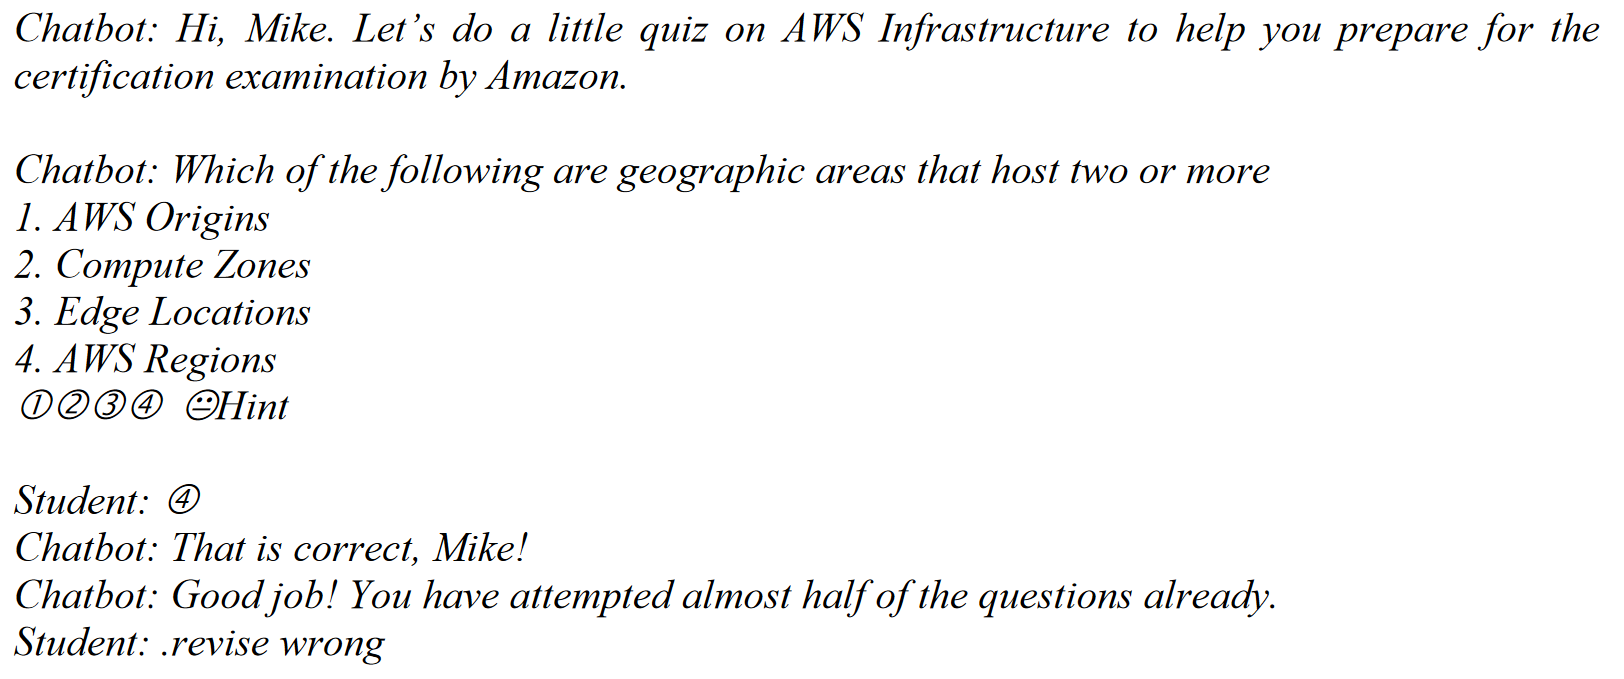
\includegraphics[width=16cm]{figuras/chatbot-wong.png}
    }{
		\Fonte{\citeonline{wong2022}.}
	}
\end{figure}

O questionário mostrou que a maioria dos alunos (de 70\% a 85\%) responderam positivamente para as afirmativas que colocavam o chatbot melhor que o quiz online em vários aspectos. Entretanto, um pouco mais da metade dos alunos (58\%) indicou que eles levaram mais tempo para completar o chatbot que o quiz online. Assim, os beneficiados com esse estudo são professores e alunos, visto que os alunos conseguem obter assistência imediata sobre o conteúdo acadêmico ao acessar o chatbot, e os professores conseguem obter um \textit{feedback} atualizado de como anda o aprendizado dos seus discentes por meio dos resultados coletados pelo chatbot.
\section{Effectiveness of an Adaptive Learning Chatbot on Student's Learning Outcomes Based on Learning Styles \cite{kaiss2023}}
\label{sec:kaiss2023}

Sites populares de educação online como o Moodle são fontes de material para estudantes de diferentes experiências e necessidades acadêmicas. Entretanto, sem um acompanhamento apropriado, os usuários desses sites podem encontrar dificuldades em escolher os materiais apropriados para estudar, visto que eles podem oferecer uma ampla variedade de recursos \apud{kaiss2023}{udupi2016}. Assim, surge a necessidade de um sistema educacional adaptativo capaz de prover recursos pertinentes para o aprendizado dos alunos durante o processo educacional. Nesse sentido, no artigo, foi explorada a aplicação de uma ferramenta de conversação inteligente.

Sistemas educacionais adaptativos tiveram um aumento de popularidade e de influência com o passar das últimas décadas. Eles podem proporcionar instruções e recomendações de recursos educacionais com base nos diferentes níveis de conhecimento, interesses, objetivos e características pessoais dos usuários. Desse modo, para que os sistemas mencionados anteriormente possam operar adaptativamente com base nas individualidades dos seus usuários, uma direção de pesquisa que tem ganhado popularidade nos últimos tempos faz uso de estilos de aprendizado \apud{kaiss2023}{hasibuan2016}. Esses estilos de aprendizagem são formas predominantes pelas quais os alunos focam, processam, absorvem e retêm novas informações \apud{kaiss2023}{pashler2008}.

Modelos de estilos de aprendizado têm provado seu impacto na otimização do aprendizado acadêmico \apud{kaiss2023}{cruz2013}. No entanto, dadas as grandes mudanças e a liberdade da aquisição de conhecimento trazida pelo ensino online, teorias clássicas baseadas em ambientes tradicionais, sistemáticos e lineares de ensino podem não ser totalmente apropriadas para esse novo formato de ensino. Apesar de muitas pessoas ignorarem o fato de que o comportamento e o estilo de aprendizado dos estudantes variam da forma tradicional de ensino para o online, um crescente número de pesquisadores têm aplicado modelos de estilos de aprendizado no ensino online. Entretanto, a quantidade de estudos voltados para estilos online de aprendizado ainda é baixa, e na sua maioria, os modelos ainda estão na fase de criação.

Ao longo do tempo, diversos modelos de estilos de aprendizado foram propostos \apud{kaiss2023}{felder1988,honey1992,dunn1990,pask2011}. Para o desenvolvimento do sistema apresentado pelo artigo foi utilizado o modelo de Felder e Silverman (FSLSM). A escolha desse modelo se deu por conta de ser o modelo mais utilizado em sistemas educacionais, devido a ser possível quantificar o estilo de aprendizado dos alunos por meio dele. Além disso, para \apud{kaiss2023}{carver1999,garcia2007}, ele é considerado o modelo mais adequado a ser utilizado em sistemas educacionais adaptativos, ao passo de também ser de fácil implementação \apud{kaiss2023}{lu2007,hwang2013}.

O modelo FSLSM adotado caracteriza o estilo de aprendizado de cada aluno ao longo de quatro dimensões. A dimensão de processamento (Ativa/Reflexiva), diz respeito ao processamento da informação. Um estudante ativo prefere trabalhar em grupo e experimentar mais, já um estudante reflexivo prefere refletir, seja sozinho ou com uma companhia familiar. A dimensão de recepção (Visual/Verbal) é destinada à apresentação da informação. Um aluno visual gosta mais de apresentações visuais como imagens, diagramas e fluxogramas, já um aluno verbal tende a escolher apresentações orais e textuais. A dimensão de entendimento (Sequencial/Global) está relacionada à forma de organizar e progredir na compreensão da informação. Um estudante sequencial pensa de forma linear e aprende de formal incremental por meio de pequenos passos, em contraste do estudante global, que têm um pensamento sistemático e aprende em grandes saltos. A dimensão de percepção (Sensitiva/Intuitiva) trabalha sobre a percepção e assimilação da informação. Um aluno sensitivo possui um pensamento concreto, além de ser prático e compromissado com fatos e procedimentos, em contrapartida do aluno intuitivo, que é adepto da inovação e do pensamento conceitual.

Como parte do modelo FSLSM, também há um questionário composto de 44 perguntas que são usadas para determinar o estilo de aprendizado de cada aluno com base nas respostas fornecidas a ele. Assim, é possível classificar de maneira prévia cada estudante antes de eles usarem de fato um sistema adaptativo, resolvendo assim alguma problemática que aconteceria caso eles utilizassem o sistema sem que houvesse nenhuma informação sobre o estilo de aprendizado que eles possuem.

Como proposta de sistema educacional adaptativo, no artigo é desenvolvido um chatbot chamado \textit{LearningPartnerBot}, que possui a capacidade de recomendar em tempo real recursos educacionais, com base no estilo de aprendizado de cada aluno. Pensando na facilidade do acesso dos discentes a esse chatbot, ele foi construído sobre a plataforma Moodle, devido a ela ser uma das mais utilizadas na internet, além de estar disponível em uma ampla variedade de dispositivos, e de ser facilmente adaptável e extensível.

Na Figura \ref{fig:architecture-kaiss}, é apresentada a arquitetura da abordagem explorada como sistema educacional adaptativo. Conforme mencionado anteriormente, para os novos usuários da plataforma, é aplicado o questionário do modelo FSLSM com o intuito de classificar seu estilo de aprendizado preferido. Após isso, o resultado é persistido em uma base de dados dedicada aos dados dos alunos, que será consumida por um módulo do sistema responsável por recomendar recursos educacionais com base na preferência do usuário. E nesse contexto, a interação do discente com esse módulo de recomendação é intermediada pelo chatbot \textit{LearningPartnerBot} integrado na plataforma Moodle. Vale ressaltar que, para o processamento de linguagem natural das mensagens enviadas para o chatbot pelos alunos, é utilizada uma versão de código aberto do Framework DialogFlow da Google, que permite que as solicitações em linguagem natural sejam convertidas em um formato computacionalmente legível para o módulo de recomendações.

\begin{figure}[ht] 
   	\captionsetup{width=16cm}
	\Caption{\label{fig:architecture-kaiss} Arquitetura do sistema adaptativo desenvolvido}
	\UFCfig{}{
        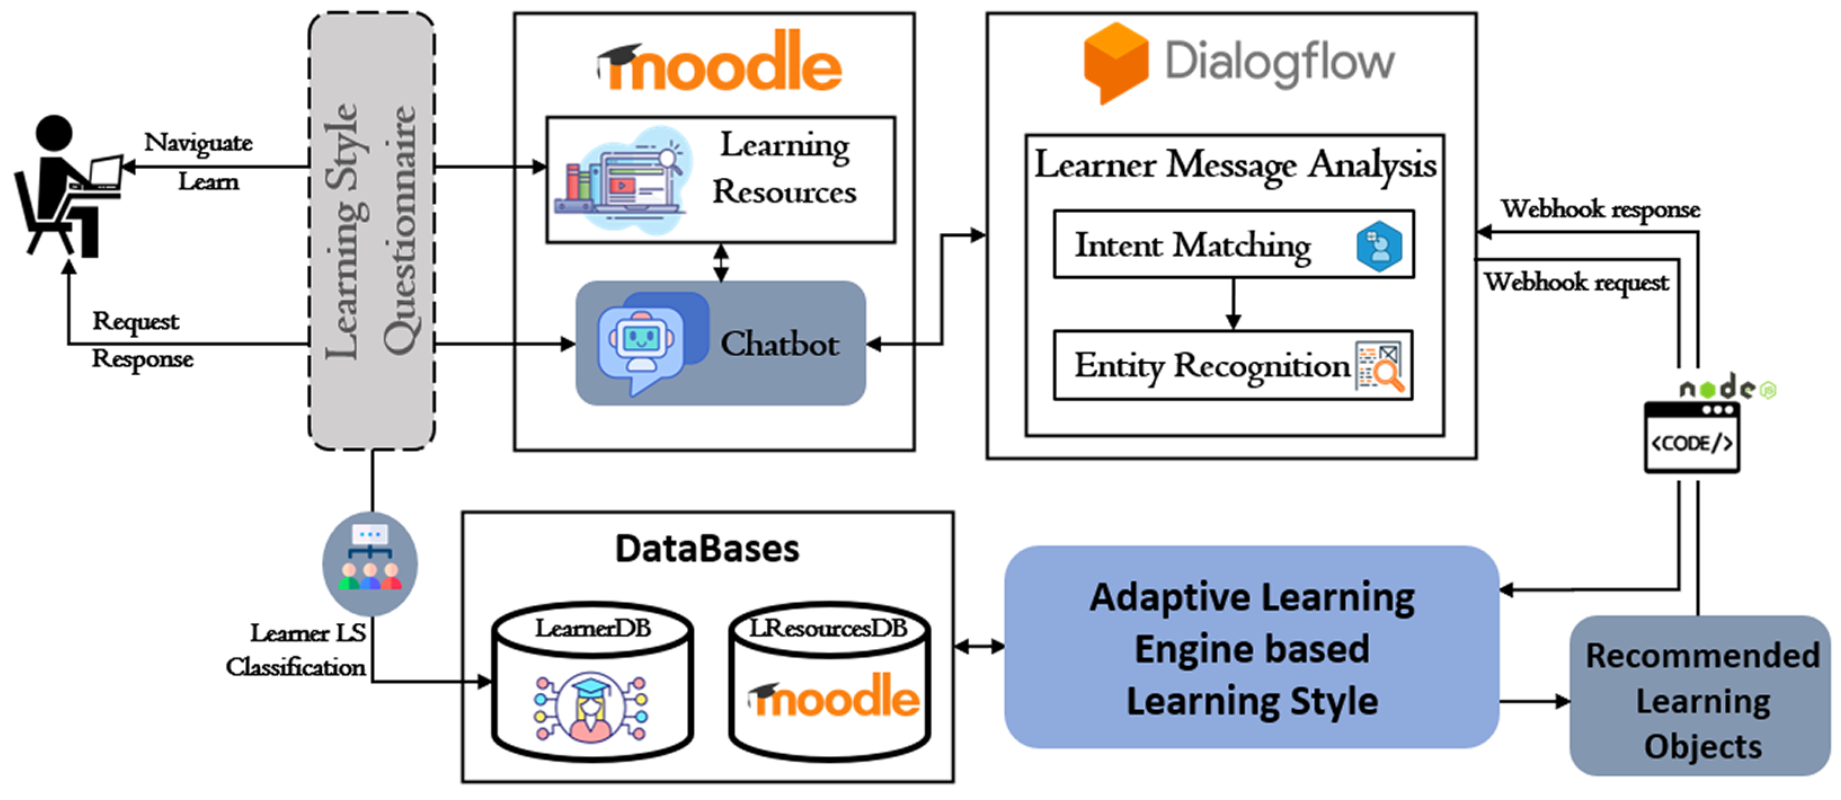
\includegraphics[width=16cm]{figuras/architecture-kaiss.png}
    }{
		\Fonte{\citeonline{kaiss2023}.}
	}
\end{figure}

Na fase de experimentação, a abordagem desenvolvida foi aplicada em uma disciplina de programação em linguagem C, para alunos do primeiro ano dos cursos de Software Engineering and Distributed Computing Systems (GLSID) e Big Data and Cloud Computing Engineering (BDCC) da escola de ensino superior marroquina Ecole Normale Supérieure de l’Enseignement Technique de Mohammedia (ENSET). A população total do estudo era de 71 discentes (Sendo 52 homens e 19 mulheres), na faixa etária de 20 a 21 anos. Durante essa etapa, os estudantes puderam usar o chatbot livremente pelo período de duas semanas e no dispositivo de sua preferência.

Na Figura \ref{fig:visual-style-recommendations-kaiss}, é mostrado um exemplo de recomendação de recurso educacional para caso o aluno tenha um estilo de aprendizado visual, em que por exemplo, ao clicar em um dos materiais fornecidos, ele será redirecionado para um conteúdo em formato de vídeo. Já no exemplo da Figura \ref{fig:verbal-style-recommendations-kaiss}, são apresentadas recomendações para caso o aluno possua um estilo textual, em que os recursos recomendados estão na forma de texto, de documentos em PDF e de apresentações em slides. A lista de recomendações dadas pelo chatbot são sempre clicáveis para facilitar o redirecionamento e a pesquisa dentro do Moodle.

\begin{figure}[ht] 
   	\captionsetup{width=16cm}
	\Caption{\label{fig:visual-style-recommendations-kaiss} Exemplo de recomendação para o estilo de aprendizado visual}
	\UFCfig{}{
        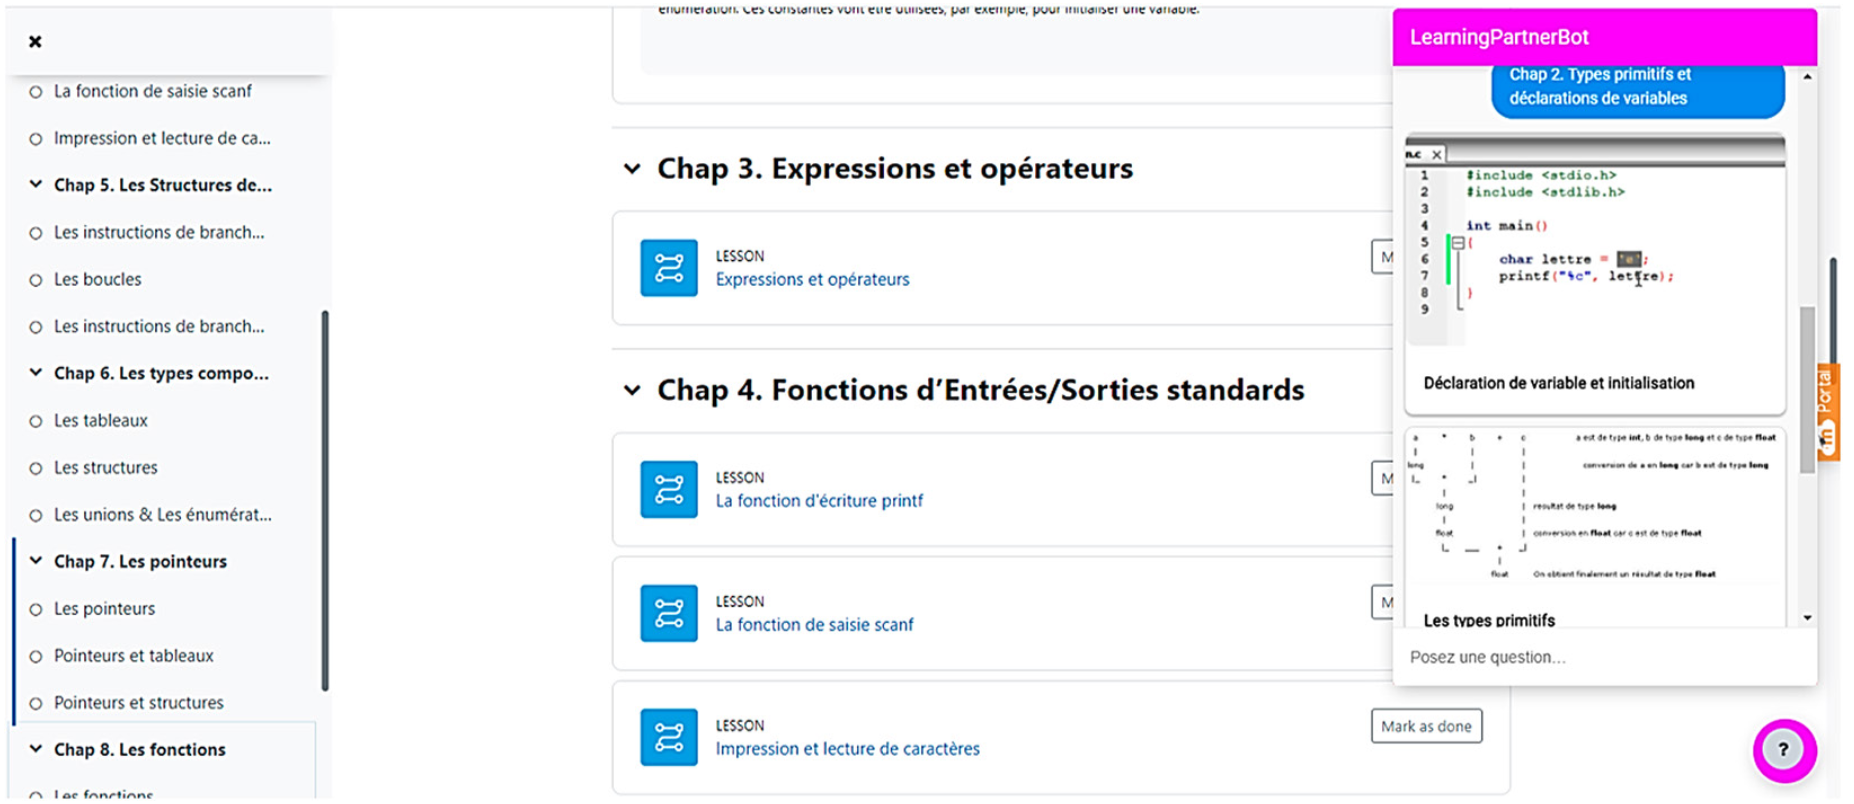
\includegraphics[width=16cm]{figuras/visual-style-recommendations-kaiss.png}
    }{
		\Fonte{\citeonline{kaiss2023}.}
	}
\end{figure}

\begin{figure}[ht] 
   	\captionsetup{width=16cm}
	\Caption{\label{fig:verbal-style-recommendations-kaiss} Exemplo de recomendação para o estilo de aprendizado textual}
	\UFCfig{}{
        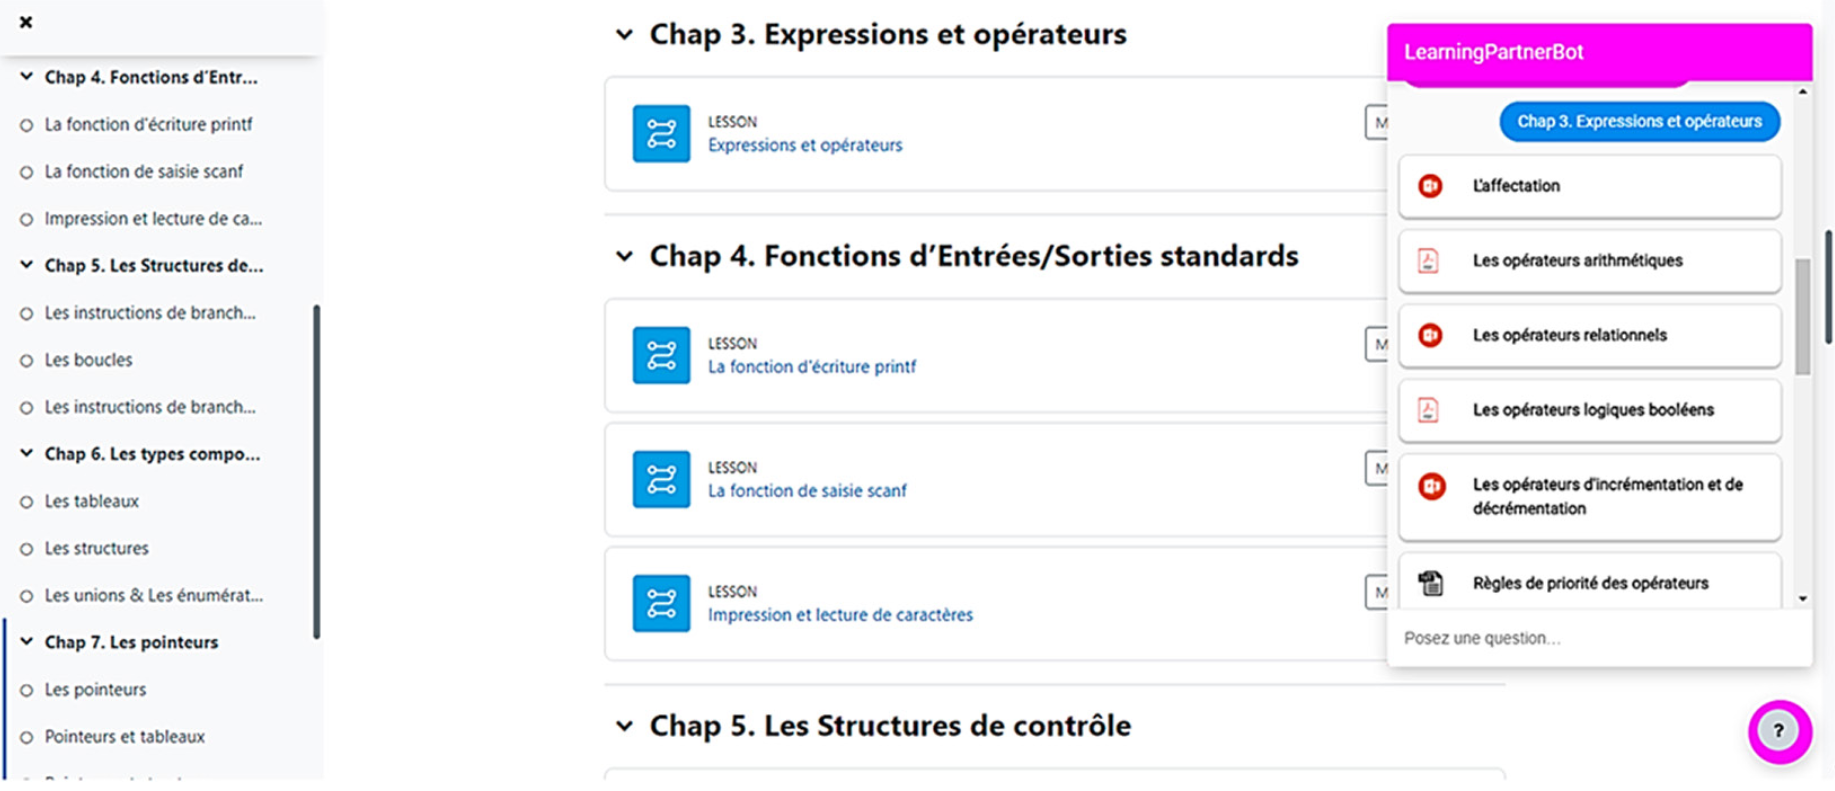
\includegraphics[width=16cm]{figuras/verbal-style-recommendations-kaiss.png}
    }{
		\Fonte{\citeonline{kaiss2023}.}
	}
\end{figure}

Antes do uso do chatbot pelos alunos, foi aplicado um pré-teste com o intuito de avaliar o nível de conhecimento que eles possuíam antes do experimento. Esse teste mostrou que 61\% deles estavam no nível iniciante e 39\% no nível intermediário. No pós-teste, os resultados obtidos mostraram que 45\% dos estudantes continuaram no nível iniciante, 49\% no intermediário e 6\% no avançado. Na Figura \ref{fig:results-kaiss}, é feito um comparativo dos dados obtidos, onde é possível perceber que a quantidade de alunos no nível iniciante teve uma diminuição de 16\%, ao passo que no nível intermediário teve um aumento de 10\%, além de que, também apareceram alunos considerados de nível avançado (6\%).

\begin{figure}[ht] 
   	\captionsetup{width=16cm}
	\Caption{\label{fig:results-kaiss} Comparação dos resultados entre o pré e o pós teste dos participantes}
	\UFCfig{}{
        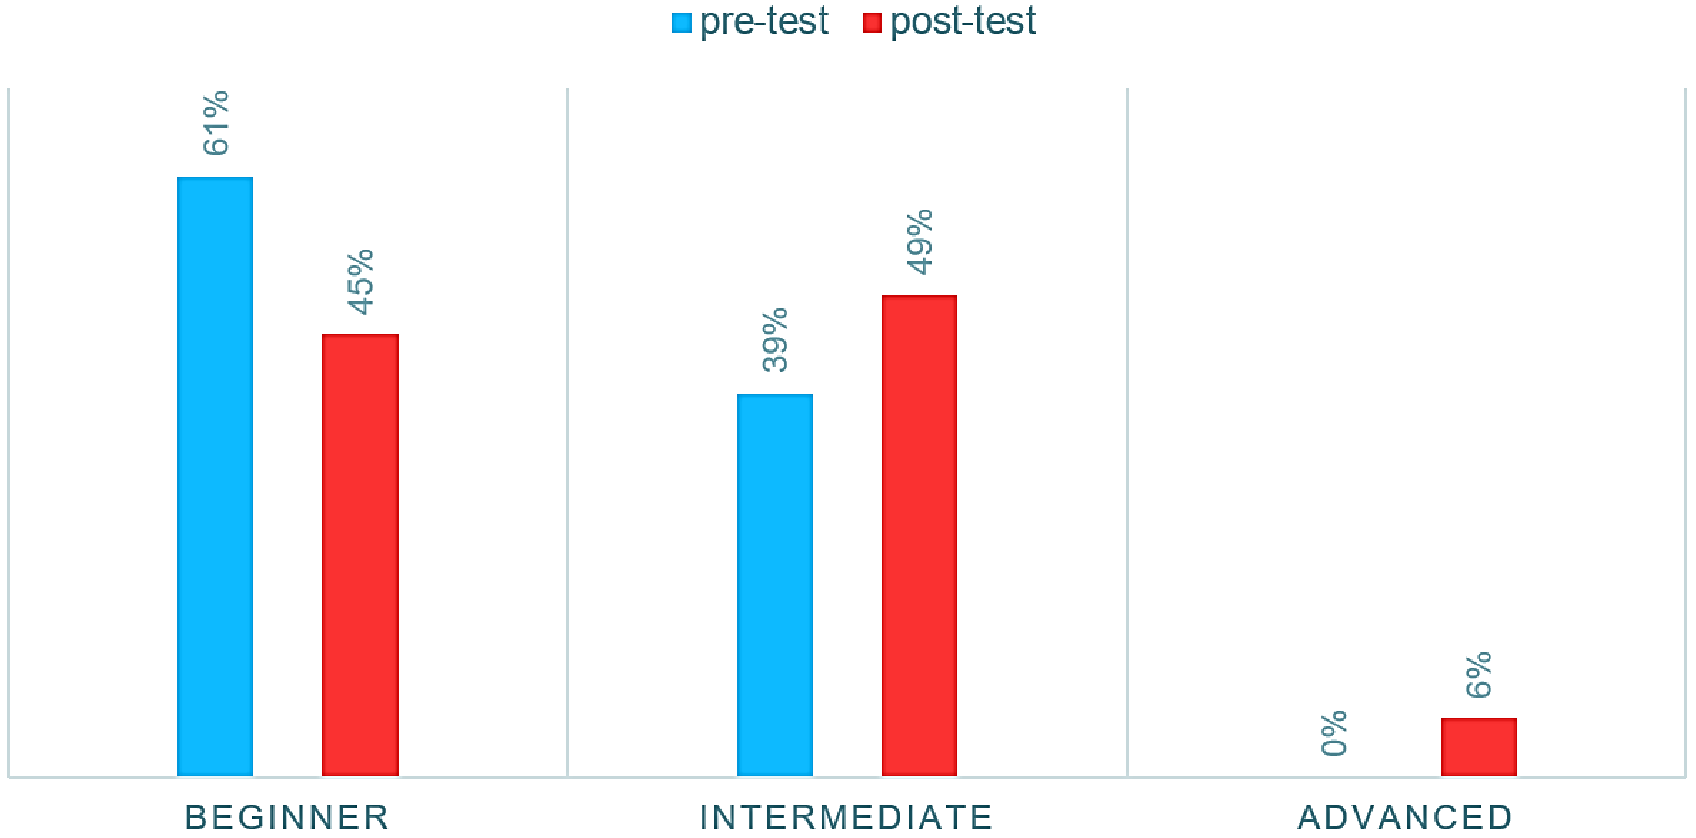
\includegraphics[width=16cm]{figuras/results-kaiss.png}
    }{
		\Fonte{\citeonline{kaiss2023}.}
	}
\end{figure}

Por fim, para avaliar a satisfação dos participantes da pesquisa em relação à abordagem proposta, após o pós-teste, foram feitas a eles as seguintes perguntas: "As recomendações apresentadas pelo \textit{LearningPartnerBot} foram úteis no processo de aprendizado?" e "Como você classifica a sua experiência geral utilizando o \textit{LearningPartnerBot}?". Os resultados coletados por essas perguntas estão apresentados na Tabela \ref{tab:results-kaiss}, que mostra a alta satisfação que os discentes tiveram com o uso do sistema educacional adaptativo construído.

\begin{table}[ht]
	\captionsetup{width=13cm}
	\Caption{\label{tab:results-kaiss} Satisfação dos participantes em relação à abordagem proposta}
	\IBGEtab{}{
		\begin{tabular}{lrrr}
			\toprule
            & Pouco interessante & Interessante & Muito interessante \\
			\midrule
			Satisfação das recomendações & 2\% & 25\% & 73\% \\
			Satisfação do uso do chatbot & 0\% & 9\% & 91\% \\
			\bottomrule
		\end{tabular}
	}{
	\Fonte{\citeonline{kaiss2023}}
}
\end{table}
\section{Rasa: Open Source Language Understanding and Dialogue Management \cite{bocklisch2017}}
\label{sec:bocklisch2017}

No campo de estudo da interação humano-computador, há uma procura por formas mais naturais de adicionar automações na vida cotidiana. Nesse contexto, é bastante difundido o uso de sistemas conversacionais, e dentre alguns dos mais conhecidos estão a Siri da Apple, a Alexa da Amazon e a Cortana da Microsoft.

No artigo de \citeonline{bocklisch2017}, são apresentadas as ferramentas Rasa NLU e Rasa Core, que são bibliotecas de código aberto para a linguagem Python focadas, respectivamente, em processamento de linguagem natural e gerenciamento de diálogo. O intuito é facilitar a construção de sistemas conversacionais, com gerenciamento de diálogo baseado em aprendizado de máquina e processamento de linguagem natural, para desenvolvedores que não precisam ser necessariamente especialistas nessas áreas.

A API do Rasa utiliza ideias implementadas em outras bibliotecas de aprendizado de máquina, como herança estrita do \textit{scikit-learn} \apud{bocklisch2017}{chollet2015} e diferentes implementações de back-end do \textit{Keras} \apud{bocklisch2017}{pedregosa2011}.

A classificação de textos é vagamente baseada na abordagem \textit{fastText} \apud{bocklisch2017}{joulin2016}. As sentenças são representadas pelo agrupamento de vetores de palavras para cada token constituinte. Usando \textit{embeddings} (representações de valores ou objetos projetados para serem consumidos por modelos de aprendizado de máquina) de palavras pré-treinadas como \textit{GloVe} \apud{bocklisch2017}{pennington2014}, os classificadores de intenção são notavelmente mais robustos às variações da linguagem do que quando treinados com apenas alguns exemplos de cada intenção.

O Rasa é projetado com uma arquitetura modular. Desse modo, é possível integrá-lo facilmente com outros sistemas. Por exemplo, o Rasa Core pode ser usado como um gerenciador de diálogos em conjunto com outros serviços de NLU que não sejam o Rasa NLU. Embora eles sejam implementados em Python, ambos os serviços podem ser expostos via rede, permitindo a utilização deles em projetos feitos em outras linguagens de programação.

Na Figura \ref{fig:architecture-rasa}, é demonstrada graficamente a série de passos feitos pelo Rasa quando uma nova mensagem é recebida. Vale ressaltar que o passo 1 é feito pelo Rasa NLU, enquanto os demais são realizados pelo Rasa Core. No passo 1, a mensagem é recebida e passada para um interpretador (por exemplo, Rasa NLU) para extrair a intenção, entidades e qualquer outra informação estruturada. No passo 2, o \textit{Tracker} é notificado que uma nova mensagem foi recebida, e armazena o estado da conversa em um banco de dados. Nos passos 3 e 4, o estado atual da conversa é passado para o objeto \textit{Policy}, que será responsável por escolher a próxima ação. No passo 5, a ação escolhida é registrada no \textit{Tracker}. No passo 6, a ação é executada.

\begin{figure}[ht] 
   	\captionsetup{width=16cm}
	\Caption{\label{fig:architecture-rasa} Arquitetura do Rasa}
	\UFCfig{}{
        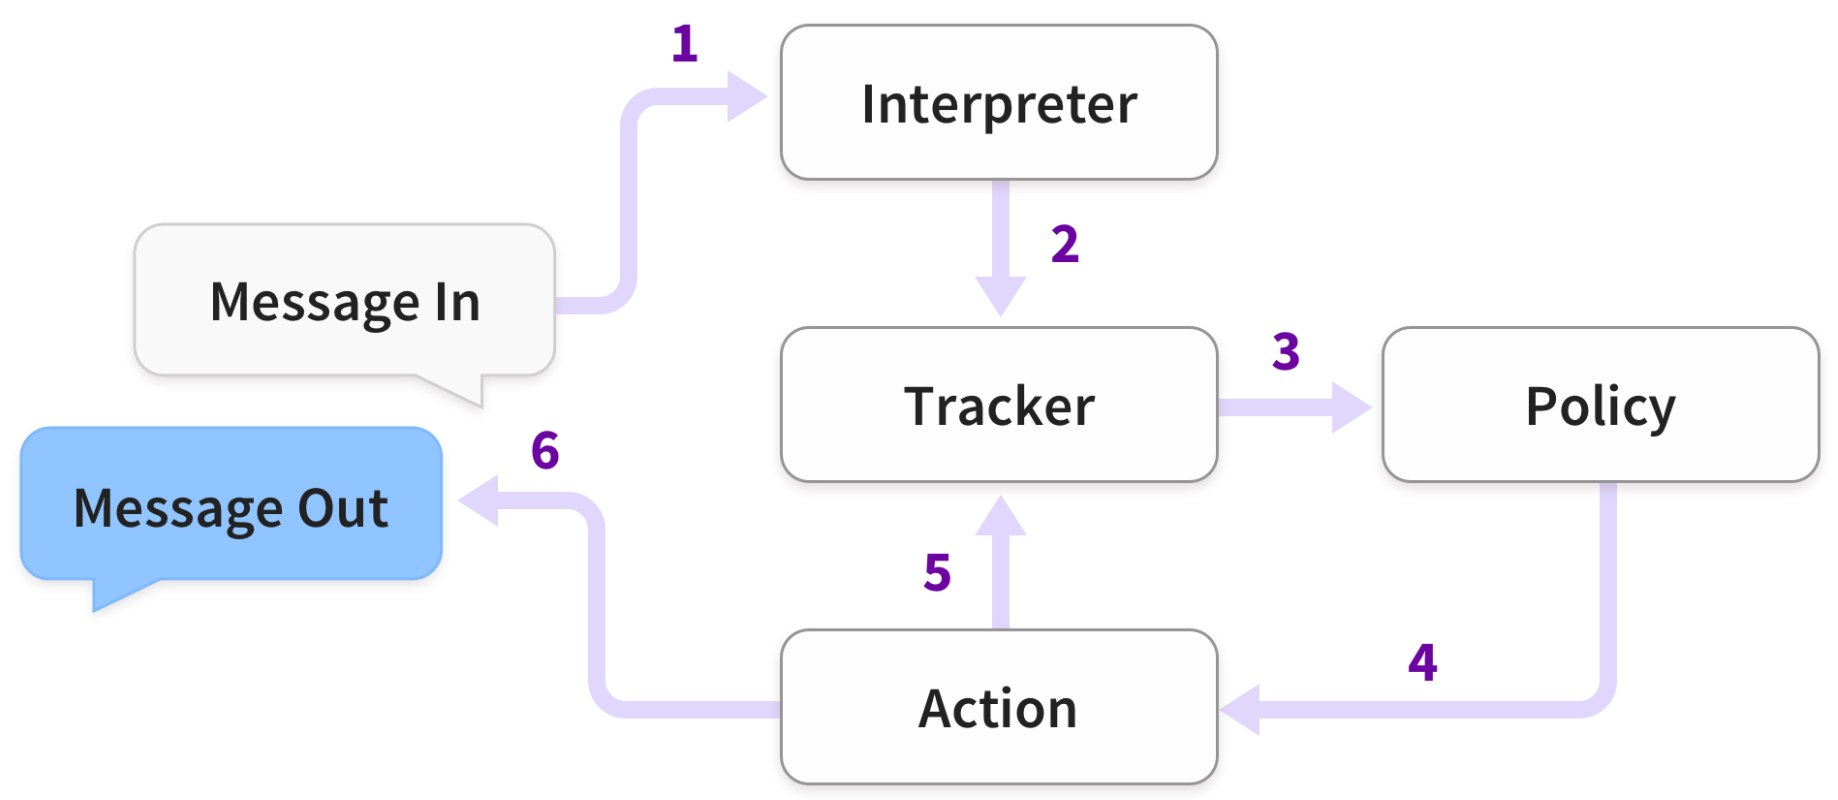
\includegraphics[width=16cm]{figuras/architecture-rasa.png}
    }{
		\Fonte{\citeonline{bocklisch2017}.}
	}
\end{figure}

O estado do diálogo é persistido em um objeto \textit{Tracker}, sendo ele único por seção de conversa. Além disso, ele é o único componente do sistema que possui estado. O \textit{Tracker} registra todos os eventos que levaram a aquele estado e que ocorreram durante a conversa. O estado da conversa pode ser reconstruído a partir desses eventos.

No Rasa, o problema de gerenciamento de diálogo é tratado como um problema de classificação. A cada iteração, o Rasa Core prevê qual será a próxima ação a ser tomada com base em uma lista predefinida de ações. Uma ação pode ir desde uma mensagem a ser enviada para o usuário até a execução de uma função arbitrária. Na execução da ação, é passada uma instância do objeto \textit{Tracker} da sessão, permitindo assim que a ação tenha acesso a qualquer informação relevante coletada previamente no diálogo.

Em adição ao aprendizado supervisionado, o Rasa Core fornece uma abordagem que permite que os desenvolvedores apliquem correções durante o seu treinamento, como exemplificado na Figura \ref{fig:rasa-training-correction}, em que após o usuário fornecer a entrada ``/greet'' destacada em verde, o Rasa Core escolheu a ação ``utter\_ask\_howcanhelp'' destacada em vermelho, e questionou se essa ação era correta com base na entrada. Caso seja informado que a ação é incorreta, será mostrada a lista de possíveis ações, bem como cada probabilidade associada a elas pelas políticas da conversa (Figura \ref{fig:rasa-actions}).

\begin{figure}[ht] 
   	\captionsetup{width=16cm}
	\Caption{\label{fig:rasa-training-correction} Exemplo de correção durante o treinamento do Rasa}
	\UFCfig{}{
        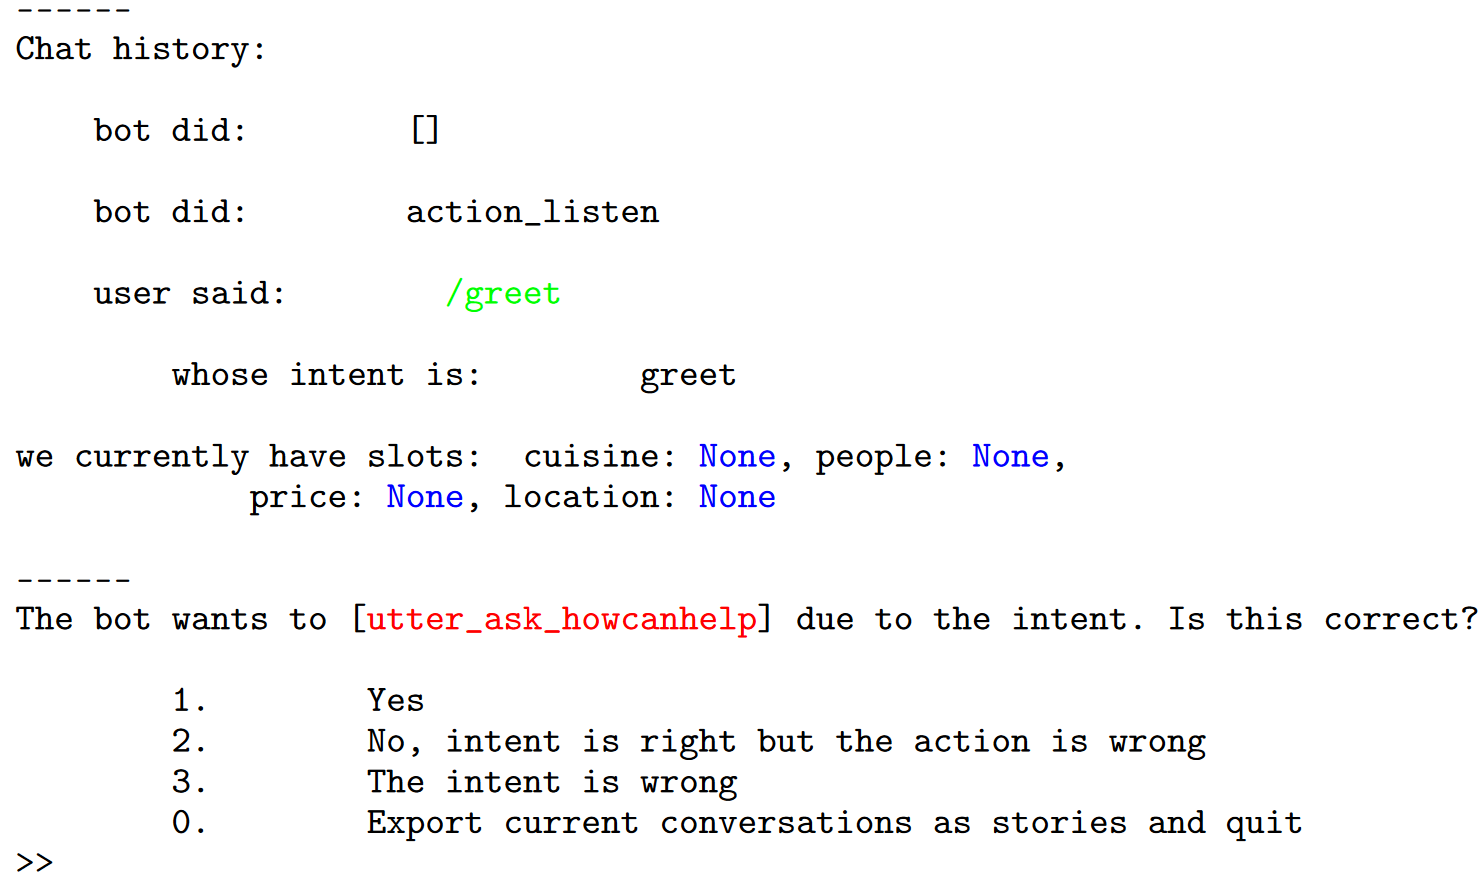
\includegraphics[width=16cm]{figuras/rasa-training-correction.png}
    }{
		\Fonte{\citeonline{bocklisch2017}.}
	}
\end{figure}

\begin{figure}[ht] 
   	\captionsetup{width=16cm}
	\Caption{\label{fig:rasa-actions} Exemplo de escolha da próxima ação do Rasa durante a correção}
	\UFCfig{}{
        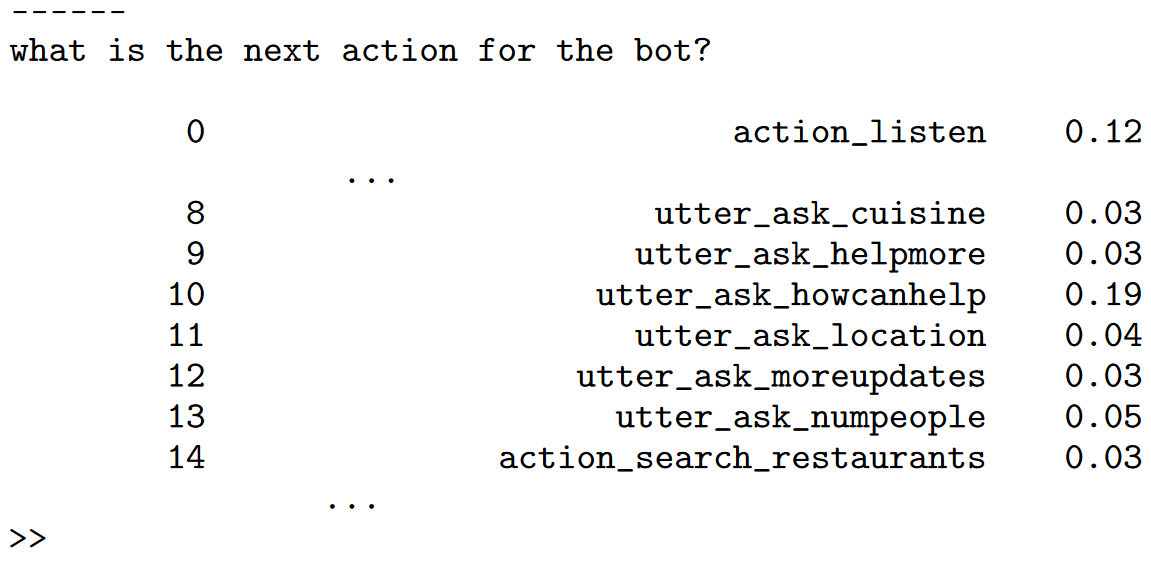
\includegraphics[width=16cm]{figuras/rasa-actions.png}
    }{
		\Fonte{\citeonline{bocklisch2017}.}
	}
\end{figure}

Tanto o Rasa NLU quanto o Rasa Core estão sendo desenvolvidos ativamente. Eles são plataformas gratuitas para a aplicação de pesquisas em modelos conversacionais de inteligência artificial por desenvolvedores que não precisam ser especialistas nessas áreas, e portanto não há previsão de serem finalizados.
\section{Toward an eclectic and malleable multiagent educational assistant \cite{briel2021}}
\label{sec:briel2021}

%Agentes conversacionais são sistemas capazes de processar e responder linguagem natural. Eles evoluíram com o passar dos anos, indo desde um meio para passar no Teste de Turing até chatbots que possuem um objetivo utilitário, como suporte ao cliente \apud{briel2021}{cui2017} e tutoria \apud{briel2021}{wang2013}. Uma distinção pode ser feita entre agentes de domínio aberto e domínio fechado, enquanto os de domínio aberto são capazes de manter uma conversa sobre diversos assuntos, os de domínio fechado são mais orientadas à tarefas e tendem a conseguir retornar informações para uma variedade de solicitações.

Chatbots de domínio fechado são frequentemente limitados em funcionalidade, seja por serem capazes de conversar sobre apenas um domínio específico, responder apenas à perguntas simples ou buscar arquivos. Apesar dessas limitações, existe uma ampla variedade de funcionalidades possíveis que um agente pode oferecer, podendo até ser um assistente educacional e fornecer recomendações de materiais acadêmicos.

Um sistema que é capaz de executar todas essas funcionalidades acima simultaneamente se destacaria dos demais agentes que possuem apenas uma única função. Com base nas necessidades dos alunos, funções diferentes, como fornecer links, resumos ou conteúdos abrangendo várias bases de conhecimento, podem facilitar o aprendizado individual. Assim, para atender a essas necessidades, no artigo de \citeonline{briel2021}, é proposto um framework multiagente chamado JuggleChat, formado internamento por vários chatbots e outros componentes relacionados, que possui foco na diversidade de funções do chatbot e não apenas no conhecimento de domínio fechado.

Conforme descrito na Figura \ref{fig:architecture-briel}, a arquitetura do JuggleChat é constituída por uma interface do usuário, um módulo de extração da intenção da mensagem, um alocador de chatbots e vários chatbots internos. Com isso, no fluxo de dados, a entrada do usuário é processada pelo módulo de extração da intenção. Em seguida, a intenção e a entrada são passadas para o alocador de chatbots que, com base na intenção, define para qual chatbot interno será direcionada a mensagem. Por fim, o respectivo chatbot processa a mensagem e gera uma resposta, que é então enviada para o usuário.

\begin{figure}[ht] 
   	\captionsetup{width=16cm}
	\Caption{\label{fig:architecture-briel} Arquitetura do JuggleChat}
	\UFCfig{}{
        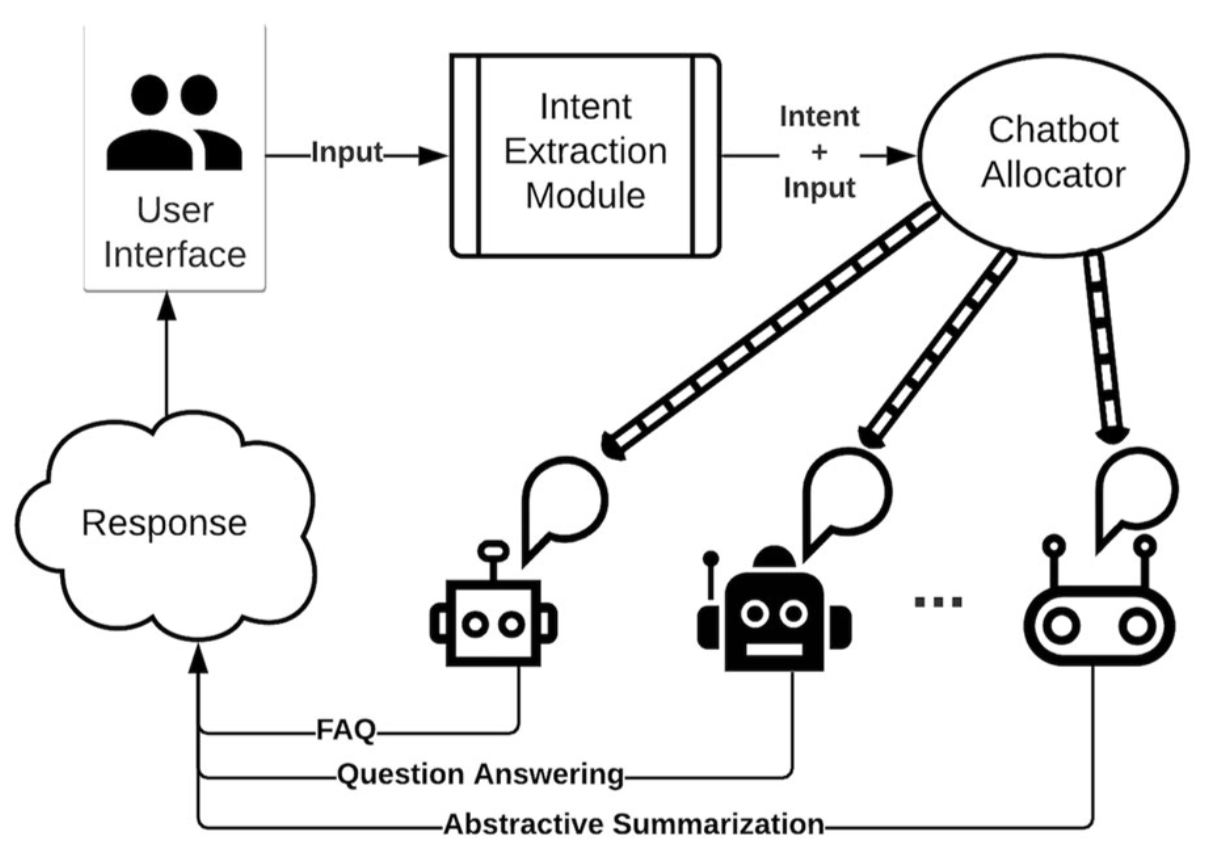
\includegraphics[width=16cm]{figuras/architecture-briel.png}
    }{
		\Fonte{\citeonline{briel2021}.}
	}
\end{figure}

A arquitetura desse estudo foi planejada usando bibliotecas e componentes de código aberto. A interface do usuário para o processamento de entradas e entrega de respostas foi construída usando React e TypeScript, com seu backend constituído por um servidor Express que se comunica com um banco de dados PostgreSQL. Uma instância do Rasa foi utilizada para o módulo de extração da intenção do usuário.

Os dois principais objetivos do experimento foram determinar a eficiência do JuggleChat como ferramenta de auxílio aos estudantes durante o aprendizado, e entender como os participantes se sentem durante a interação com o chatbot e como eles percebem sua precisão e utilidade.

Quatro grupos de cem participantes cada foram usados para avaliar o uso do framework, e ninguém sabia da tecnologia subjacente do chatbot que estavam usando. O primeiro grupo usou apenas um chatbot baseado em respostas curtas. Já o segundo grupo usou apenas um chatbot baseado em respostas longas. O terceiro grupo usou o JuggleChat que continha os dois chatbots citados anteriormente, além de possuir um módulo de sumarização e a capacidade de enviar URLs. O quarto grupo não fez uso de chatbots. Os grupos que possuíam acesso ao chatbot foram alocados para avaliar o sistema multiagente no geral e os chatbots usados internamente, já o objetivo de ter um grupo que não fazia de uso de chatbots foi para mensurar o quanto o acesso aos chatbots afetaria a performance do teste.

Em um primeiro momento, foi passado para os participantes um conjunto de instruções indicando que eles teriam uma lição sobre informações relacionadas ao COVID-19. Caso eles fizessem parte de um dos três grupos que usariam o chatbot, também foi repassado que eles poderiam fazer cinco perguntas para um chatbot (Figura \ref{fig:conversation-briel}), depois avaliar a interação com ele (Figura \ref{fig:evaluation-briel}), e no final, realizar um questionário sobre o conteúdo (Figura \ref{fig:quiz-briel}). Os participantes que não usariam o chatbot apenas receberam a instrução que eles realizariam um questionário após o término da lição (Figura \ref{fig:quiz-briel}).

\begin{figure}[ht] 
   	\captionsetup{width=16cm}
	\Caption{\label{fig:conversation-briel} Exemplo de interação com o JuggleChat}
	\UFCfig{}{
        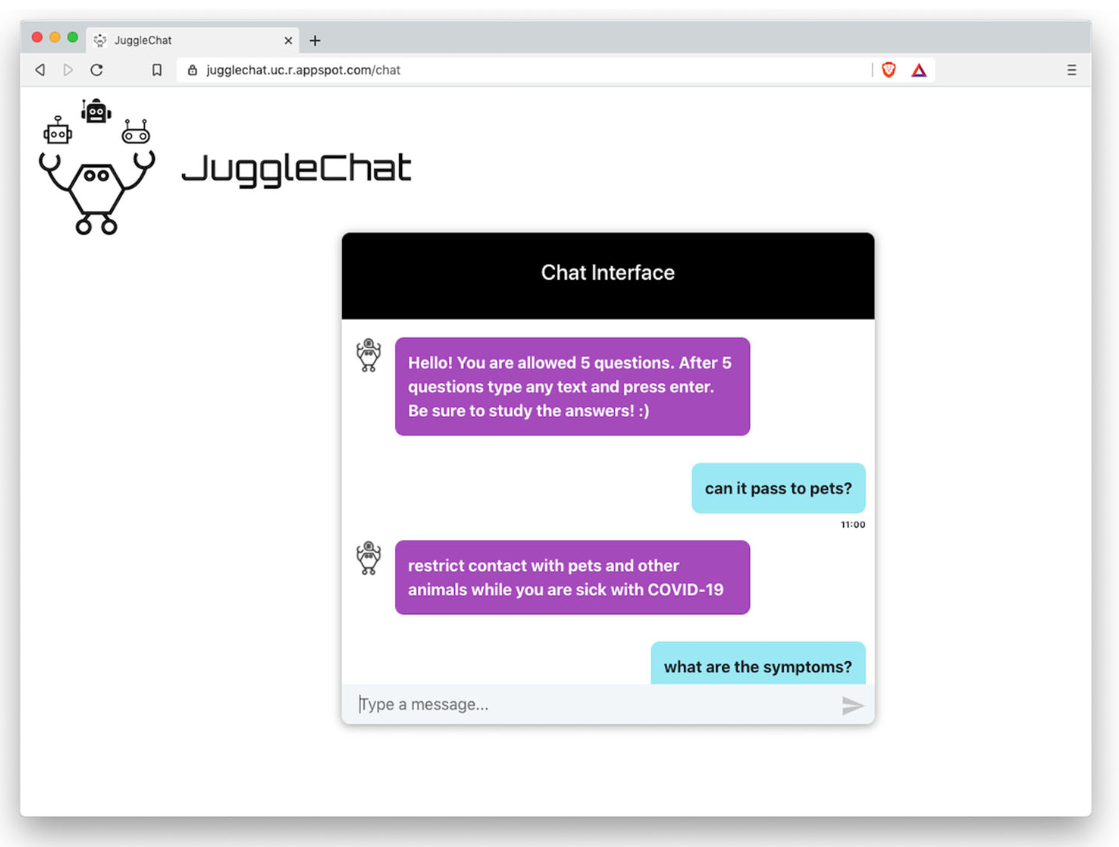
\includegraphics[width=16cm]{figuras/conversation-briel.png}
    }{
		\Fonte{\citeonline{briel2021}.}
	}
\end{figure}

\begin{figure}[ht] 
   	\captionsetup{width=16cm}
	\Caption{\label{fig:evaluation-briel} Avaliação da interação com o JuggleChat}
	\UFCfig{}{
        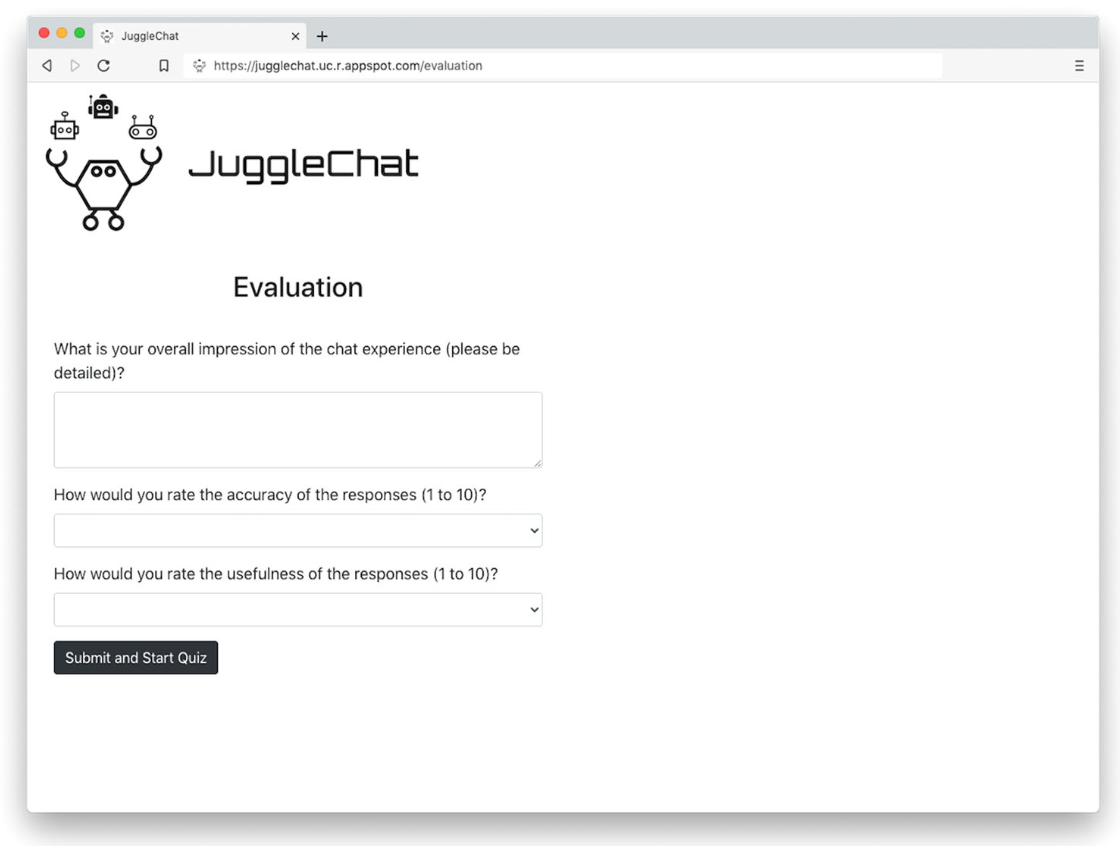
\includegraphics[width=16cm]{figuras/evaluation-briel.png}
    }{
		\Fonte{\citeonline{briel2021}.}
	}
\end{figure}

\begin{figure}[ht] 
   	\captionsetup{width=16cm}
	\Caption{\label{fig:quiz-briel} Questionário sobre o COVID-19}
	\UFCfig{}{
        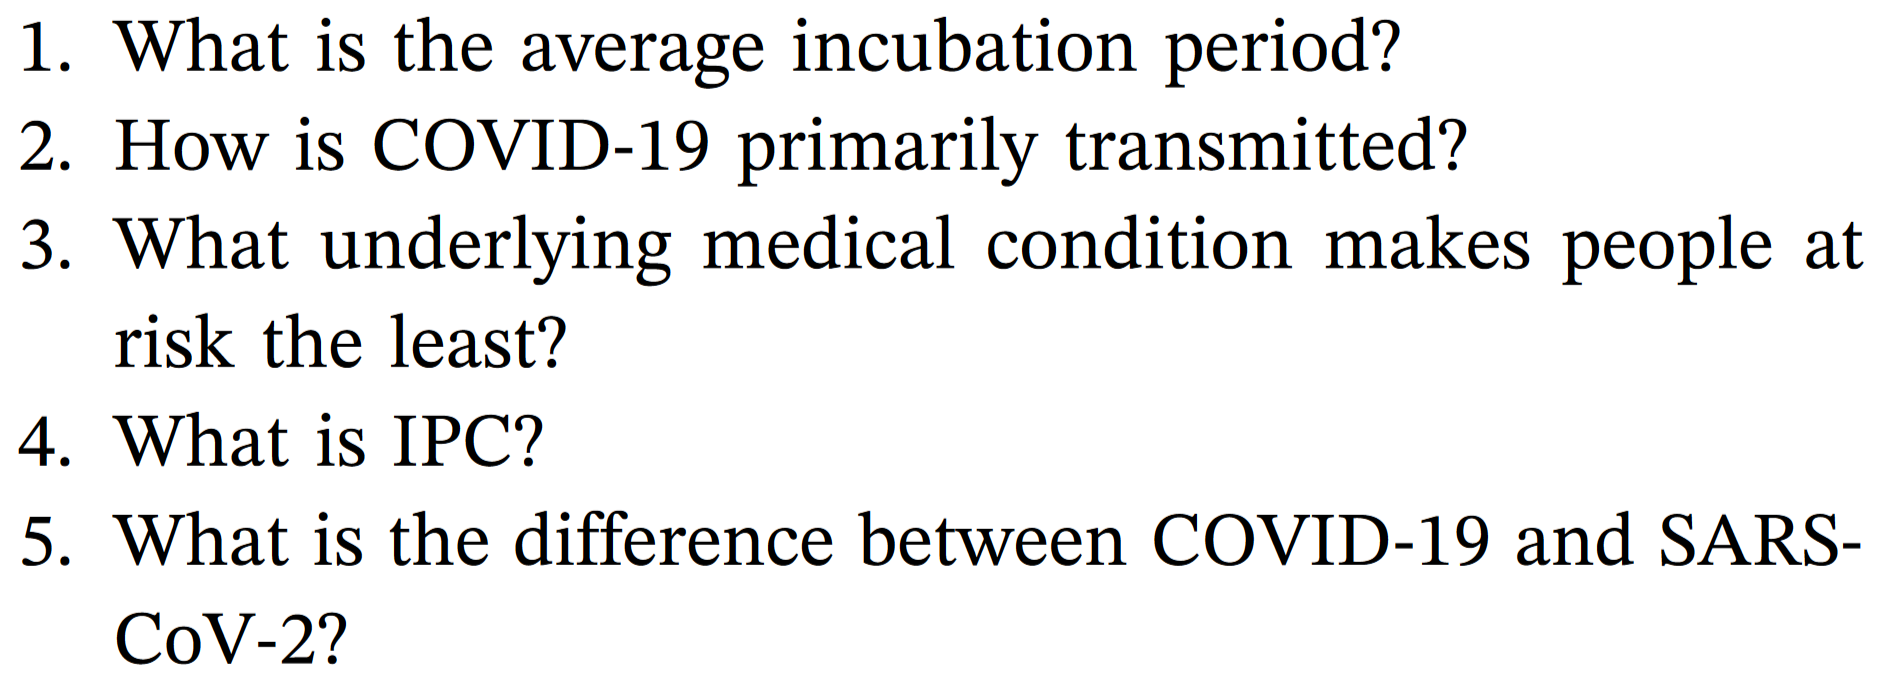
\includegraphics[width=16cm]{figuras/quiz-briel.png}
    }{
		\Fonte{\citeonline{briel2021}.}
	}
\end{figure}

Os resultados desse artigo mostraram que os participantes tiveram uma maior adesão ao chatbot baseado em respostas longas, ao passo que o chatbot baseado em respostas curtas foi avaliado como menos preciso e de menor utilidade. Por fim, o autor pontua que, diante de outros cenários de aprendizagem, essa preferência sobre o estilo do chatbot pode mudar. Assim, ele enfatiza a capacidade de adaptação do JuggleChat, devido a ele conseguir fornecer várias funcionalidades para atender às necessidades dos estudantes.

\section{Considerações finais}
\label{sec:tr-consideracoes-finais}

Neste capítulo, foi abordada uma série de trabalhos relacionados à aplicação de chatbots no contexto educacional. Com isso, foi possível identificar padrões a respeito da aplicação e do desenvolvimento de chatbots, como o uso de uma ferramenta externa para o processamento de linguagem natural \cite{kaiss2023, briel2021} e a integração com plataformas já consolidadas como interface para o chatbot \cite{kaiss2023}, que auxiliaram na elaboração da metodologia proposta deste trabalho.

Nesse sentido, a tecnologia que possui maior destaque dentre as apresentadas neste capítulo para o seguimento desse trabalho é o Rasa, especificada no artigo de \citeonline{bocklisch2017}. Com sua capacidade de processamento de linguagem natural e gerenciamento do estado do diálogo, ela é uma peça fundamental na construção do chatbot proposto neste trabalho.
	%% Em TCC 2, colocar apenas Metodologia
\chapter{Metodologia proposta}
\label{cap:metodologia}

Este capítulo descreve a proposta de uma metodologia para o desenvolvimento de um chatbot para uso em disciplinas de nível de graduação, que poderá ser utilizado, em particular, na disciplina de Cálculo Numérico do Campus da UFC em Russas.

Na Seção \ref{sec:escopo}, é apresentado o escopo da futura aplicação do chatbot proposto. Em seguida, na Seção \ref{sec:escolha-tecnologias}, são pontuadas as escolhas das principais tecnologias que serão usadas no desenvolvimento da aplicação. Por fim, na Seção \ref{sec:funcionamento-chatbot}, é descrito como será o funcionamento do chatbot, tanto na interação com o aluno quanto com o professor.

\section{Escopo de uso}
\label{sec:escopo}

O intuito inicial do desenvolvimento desse chatbot é que ele seja aplicado em turmas futuras dos cursos de graduação da Universidade Federal do Ceará, no Campus de Russas. Devido ao seu escopo não ser limitado a uma disciplina ou área do conhecimento específica, ele pode ter seu uso expandido em demais cursos e em demais universidades. Entretanto, como caso de teste, será utilizada a disciplina de Cálculo Numérico, disciplina obrigatória para os cursos de Engenharia Civil, Engenharia Mecânica e Engenharia de Produção e optativa para o curso de Ciência da Computação neste campus.

\section{Escolha de tecnologias}
\label{sec:escolha-tecnologias}

A plataforma escolhida como meio de interação com o chatbot foi o Telegram, devido a ela ser uma plataforma popular atualmente, e a possuir uma API gratuita para o desenvolvimento de chatbots. O Telegram também é facilmente integrável com o Rasa, que será usado tanto para o processamento de linguagem natural das mensagens dos usuários, quanto para o gerenciamento do estado da conversa.

Além disso, a linguagem de programação escolhida para a implementação do projeto foi Python, pois ela é uma linguagem de fácil uso e flexível e, principalmente por conta do Rasa ser implementado majoritariamente em Python, o que permite uma fácil integração entre as duas tecnologias.

Por fim, para os dados que precisam ser persistidos durante a execução do sistema, será usado um banco de dados PostgreSQL, que será hospedado junto dos demais componentes do chatbot em um servidor virtual privado.

\section{Funcionamento do chatbot}
\label{sec:funcionamento-chatbot}

O funcionamento do chatbot será baseado em receber mensagens dos alunos solicitando recomendações de conteúdo sobre tópicos da disciplina. A partir disso, com base nos conteúdos disponíveis e no histórico de conversação com o aluno, será possível respondê-lo com recursos pertinentes à sua necessidade acadêmica, recursos estes que podem variar desde textos até mídias audiovisuais. Na Figura \ref{fig:chatbot-telegram-student}, é demonstrado um protótipo da interação de um aluno com o chatbot.

\begin{figure}[ht] 
   	\captionsetup{width=16cm}
	\Caption{\label{fig:chatbot-telegram-student} Protótipo de interação com o chatbot na visão do aluno}
	\UFCfig{}{
        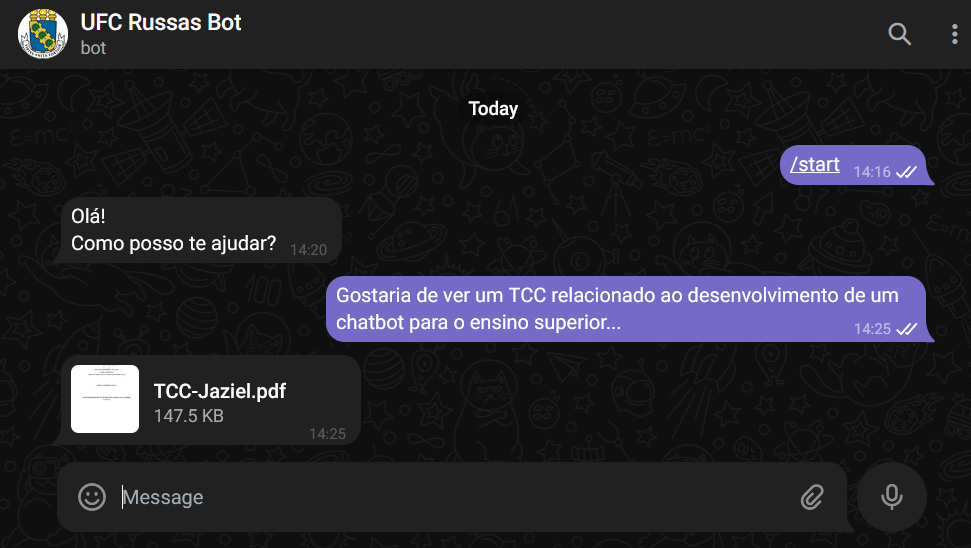
\includegraphics[width=16cm]{figuras/chatbot-telegram-student.png}
    }{
		\Fonte{Elaborado pelo autor}
	}
\end{figure}

Esses conteúdos recomendados pelo chatbot serão pré-cadastrados pelo professor da disciplina dentro da sua própria interface. Na Figura \ref{fig:chatbot-telegram-professor}, é apresentado um protótipo de como ocorrerá essa interação. É importante ressaltar que a API do Telegram não limita quais tipos de arquivos podem ser enviados, permitindo, assim, que o docente tenha uma ampla liberdade de inserir qualquer arquivo que desejar.

\begin{figure}[ht]
   	\captionsetup{width=16cm}
	\Caption{\label{fig:chatbot-telegram-professor} Protótipo de interação com o chatbot na visão do professor}
	\UFCfig{}{
        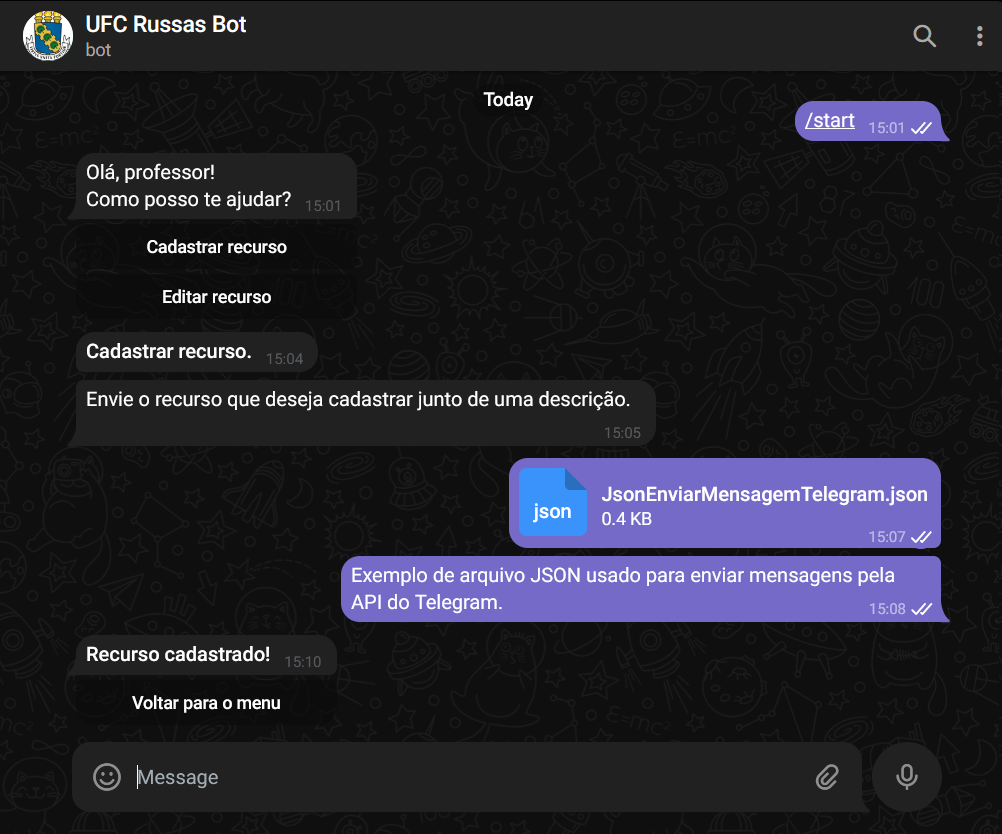
\includegraphics[width=16cm]{figuras/chatbot-telegram-professor.png}
    }{
		\Fonte{Elaborado pelo autor}
	}
\end{figure}

O acesso a diferentes funcionalidades dentro do chatbot será controlado por meio de perfis de acesso atrelados à conta do Telegram de cada usuário. Em um primeiro momento, os únicos perfis disponíveis serão o de docente e o de estudante. Caso não haja um perfil de acesso associado a uma determinada conta, será atribuído o perfil de acesso padrão, que é o de estudante.

\section{Considerações finais}
\label{sec:mp-consideracoes-finais}

Este capítulo descreveu a metodologia proposta para o desenvolvimento do chatbot que realize o objetivo geral desse trabalho. O próximo capítulo descreve sucintamente os resultados esperados com a aplicação desse chatbot.
	%\chapter{Resultados esperados}
\label{cap:resultados-esperados}

Mediante o exposto, devido à escolha do Telegram como interface do chatbot, espera-se desenvolver um ambiente de aprendizado online de fácil acesso para os alunos, aproveitando da visibilidade que a plataforma já possui, em comparação com o desenvolvimento de um site ou aplicativo que serviria como interface para uma aplicação similar à proposta neste trabalho.

Com o chatbot, almeja-se que tanto professores quanto alunos se beneficiem do seu uso em disciplinas.

Com relação aos alunos, o chatbot dará maior autonomia a eles durante o processo educacional, já que será possível obter facilmente recursos pertinentes ao conteúdo das disciplinas, o que poderia auxiliar na fixação do conteúdo em momentos extraclasse.

Como consequência, os professores também terão benefícios ao aplicar o chatbot em suas disciplinas, pois, a partir das interações com o chatbot, as dúvidas dos alunos seriam sanadas com os materiais cadastrados pelo professor, o que viria a diminuir a demanda pelo docente fora de sala de aula.
	%\chapter{Cronograma}
\label{cap:cronograma}

Com o intuito de organizar as etapas seguintes da execução deste trabalho nos próximos seis meses, foi elaborado o cronograma presente no Quadro \ref{qua:cronograma}.

\begin{quadro}[ht]
	\captionsetup{width=11.2cm}
	\Caption{\label{qua:cronograma} Cronograma de atividades do trabalho de conclusão de curso}
	\UFCqua{}{
		\begin{tabular}{|c|c|c|c|c|c|c|}
			\hline
			Atividades & Out. & Nov. & Dez. & Jan. & Fev. & Mar. \\
			\hline
			Revisão bibliográfica & \cellcolor{gray} & \cellcolor{gray} & \cellcolor{gray} & \cellcolor{gray} & \cellcolor{gray} & \\
			\hline
			Desenvolvimento da aplicação & \cellcolor{gray} & \cellcolor{gray} & \cellcolor{gray} & & & \\
			\hline
			Realização de testes & & & \cellcolor{gray} & & & \\
			\hline
			Análise dos resultados & & & \cellcolor{gray} & \cellcolor{gray} & & \\
			\hline
			Escrita do documento & & & & \cellcolor{gray} & \cellcolor{gray} & \\
			\hline
			Entrega do documento & & & & & \cellcolor{gray} & \\
			\hline
			Defesa do trabalho & & & & & & \cellcolor{gray} \\
			\hline
		\end{tabular}
	}{
		\Fonte{Elaborado pelo autor}
	}
\end{quadro}
	%\chapter{Conclusão}
\label{cap:conclusao}

Com base no que foi apresentado nesse trabalho, é possível compreender que chatbots podem ser uma ferramenta poderosa de ensino online, permitindo que professores disseminem de forma assíncrona para os alunos materiais complementares ao que foi ministrado em sala de aula, fortalecendo assim a absorção e a fixação do conteúdo.

Desse modo, espera-se que o chatbot proposto, a ser aplicado, em um primeiro momento, na disciplina de Cálculo Numérico, traga benefícios para toda a comunidade acadêmica da Universidade Federal do Ceará no Campus de Russas.
	
	%Elementos pós-textuais	
	%\bibliography{3-pos-textuais/referencias}
%	\imprimirglossario %	
	%\imprimirapendices
		% Adicione aqui os apendices do seu trabalho
		%\apendice{EXEMPLO DE APÊNDICE}
\label{ap:A}

Um apêndice é um documento elaborado pelo autor, diferentemente do anexo. Geralmente, se coloca como apêndice, questionários, códigos de programação, tabelas que tomariam muito espaço no meio do trabalho.
		%\apendice{ Questionário utilizado para}
\label{ap:B}

\begin{questao}
	\item Esta é a primeira questão com alguns itens:
		\begin{enumerate}
			\item Este é o primeiro item
			\item Segundo item
		\end{enumerate}
	\item Esta é a segunda questão:
		\begin{enumerate}
			\item Este é o primeiro item
			\item Segundo item
		\end{enumerate}
	\item Lorem ipsum dolor sit amet, consectetur adipiscing elit. Nunc dictum sed tortor nec viverra. consectetur adipiscing elit. Nunc dictum sed tortor nec viverra.
		\begin{enumerate}
			\item consectetur
			\item adipiscing
			\item Nunc
			\item dictum
		\end{enumerate}
\end{questao}

		%\apendice{ Códigos-fontes utilizados para}
\label{ap:C}

\lstinputlisting[language=C++,caption={Hello World em C++}]{figuras/main.cpp}


\begin{lstlisting}[language=Java,caption={Hello World em Java}]
public class HelloWorld {
	public static void main(String[] args) {
		System.out.println("Hello World!");
	}
}
\end{lstlisting}


		
		%\imprimiranexos
		% Adicione aqui os anexos do seu trabalho
		%\anexo{ Exemplo de um anexo}
\label{an:ex_anexo_a}

Um anexo é um documento que não foi elaborado pelo autor, ou seja, o autor apenas anexa. Anexos podem ser tabelas, mapas, diagramas, \textit{datasheets}, manuais e etc. 




		%\anexo{ Exemplo de um anexo em PDF}
\label{an:ex_anexo_b}

O autor pode anexar um \gls{PDF}, traduzido como formato portátil de documento. Veja o código fonte utilizado para anexar o arquivo ``Sikasil.pdf'' que foi colocado dentro da pasta ``anexos'' que por sua vez está dentro da pasta ``elementos-pos-textuais''. Tenha muita atenção na hora de especificar o local do arquivo. Recomenda-se não utilizar caracteres especiais para nomear pastas e, principalmente, arquivos. 

Pode-se fazer uma descrição sucinta do arquivo anexado.

%Comando para incluir um arquivo em PDF:
\includepdf[pages={-}]{3-pos-textuais/anexos/Sikasil.pdf}

		
    %\imprimirindice
    
	

\end{document}